\documentclass[12pt]{article}
\PassOptionsToPackage{numbers, compress, sort}{natbib}
\usepackage{neurips_2019}

\usepackage[utf8]{inputenc} % allow utf-8 input
\usepackage[T1]{fontenc}    % use 8-bit T1 fonts
\usepackage{hyperref}       % hyperlinks  %[implicit=false, bookmarks=false]
\usepackage{url}            % simple URL typesetting
\usepackage{booktabs}       % professional-quality tables
\usepackage{amsfonts}       % blackboard math symbols
\usepackage{nicefrac}       % compact symbols for 1/2, etc.
\usepackage{microtype}      % microtypography

\usepackage{mathtools, amsmath, amssymb, amsthm, graphicx, verbatim}
%\usepackage[thmmarks, thref, amsthm]{ntheorem}
\usepackage{color}
\definecolor{darkblue}{rgb}{0.0,0.0,0.2}
\hypersetup{colorlinks,breaklinks,
            linkcolor=darkblue,urlcolor=darkblue,
            anchorcolor=darkblue,citecolor=darkblue}
\usepackage{wrapfig}
\usepackage{subcaption}
\usepackage[colorinlistoftodos,textsize=tiny]{todonotes} % need xargs for below
%\usepackage{accents}
\usepackage{bbm}
\usepackage{xspace}

\usetikzlibrary{calc}
\newcommand{\Comments}{1}
\newcommand{\mynote}[2]{\ifnum\Comments=1\textcolor{#1}{#2}\fi}
\newcommand{\mytodo}[2]{\ifnum\Comments=1%
  \todo[linecolor=#1!80!black,backgroundcolor=#1,bordercolor=#1!80!black]{#2}\fi}
\newcommand{\raf}[1]{\mynote{green}{[RF: #1]}}
\newcommand{\raft}[1]{\mytodo{green!20!white}{RF: #1}}
\newcommand{\jessie}[1]{\mynote{purple}{[JF: #1]}}
\newcommand{\jessiet}[1]{\mytodo{purple!20!white}{JF: #1}}
\newcommand{\bo}[1]{\mynote{blue}{[Bo: #1]}}
\newcommand{\botodo}[1]{\mytodo{blue!20!white}{[Bo: #1]}}
\newcommand{\btw}[1]{}%TURN OFF FOR NOW \mytodo{gray}{#1}}
\ifnum\Comments=1               % fix margins for todonotes
  \setlength{\marginparwidth}{1in}
\fi


\newcommand{\reals}{\mathbb{R}}
\newcommand{\posreals}{\reals_{>0}}%{\reals_{++}}
\newcommand{\dom}{\mathrm{dom}}

\newcommand{\prop}[1]{\mathrm{prop}[#1]}
\newcommand{\eliccts}{\mathrm{elic}_\mathrm{cts}}
\newcommand{\eliccvx}{\mathrm{elic}_\mathrm{cvx}}
\newcommand{\elicpoly}{\mathrm{elic}_\mathrm{pcvx}}
\newcommand{\elicembed}{\mathrm{elic}_\mathrm{embed}}

\newcommand{\cell}{\mathrm{cell}}

\newcommand{\abstain}[1]{\mathrm{abstain}_{#1}}
\newcommand{\mode}{\mathrm{mode}}

\newcommand{\simplex}{\Delta_\Y}

% alphabetical order, by convention
\newcommand{\C}{\mathcal{C}}
\newcommand{\D}{\mathcal{D}}
\newcommand{\E}{\mathbb{E}}
\newcommand{\F}{\mathcal{F}}
\newcommand{\I}{\mathcal{I}}
\newcommand{\R}{\mathcal{R}}
\newcommand{\U}{\mathcal{U}}
\newcommand{\X}{\mathcal{X}}
\newcommand{\Y}{\mathcal{Y}}

\newcommand{\risk}[1]{\underline{#1}}
\newcommand{\inprod}[2]{\langle #1, #2 \rangle}%\mathrm{int}(#1)}
\newcommand{\inter}[1]{\mathring{#1}}%\mathrm{int}(#1)}
%\newcommand{\expectedv}[3]{\overline{#1}(#2,#3)}
\newcommand{\expectedv}[3]{\E_{Y\sim{#3}} {#1}(#2,Y)}
\newcommand{\toto}{\rightrightarrows}
\newcommand{\strip}{\mathrm{strip}}
\newcommand{\trim}{\mathrm{trim}}
\newcommand{\fplc}{finite-piecewise-linear and convex\xspace} %xspace for use in text
\newcommand{\conv}{\mathrm{conv}}
\newcommand{\indopp}{\bar{\mathbbm{1}}}
\newcommand{\ones}{\mathbbm{1}}
\DeclarePairedDelimiter\ceil{\lceil}{\rceil}

\newcommand{\Ind}[1]{\ones\{#1\}}

\newcommand{\hinge}{L_{\mathrm{hinge}}}
\newcommand{\ellzo}{\ell_{\text{0-1}}}
\newcommand{\ellabs}[1]{\ell_{#1}}

\DeclareMathOperator*{\argmax}{arg\,max}
\DeclareMathOperator*{\argmin}{arg\,min}
\DeclareMathOperator*{\arginf}{arg\,inf}
\DeclareMathOperator*{\sgn}{sgn}

\newtheorem{theorem}{Theorem}
\newtheorem{lemma}{Lemma}
\newtheorem{proposition}{Proposition}
\newtheorem{corollary}{Corollary}
\newtheorem{conjecture}{Conjecture}

\newtheorem{definition}{Definition}
\newtheorem{assumption}{Assumption}


\title{An Embedding Framework for Consistent Polyhedral Surrogates}
%\title{Consistent Polyhedral Surrogates via Embeddings}
%\title{Convex Surrogates via Polyhedral Losses}
\author{%
 Jessica Finocchiaro\raf{Jessie?} \\
 \texttt{jessica.finocchiaro@colorado.edu}\\
 CU Boulder
 \And
 Rafael Frongillo\\
 \texttt{raf@colorado.edu}\\
 CU Boulder
 \And
 Bo\\
 \texttt{bwag@colorado.edu}\\
 MSFT
}

\begin{document}

\maketitle

\begin{abstract}
We formalize and study the natural approach of designing convex surrogate loss functions via embeddings for problems such as classification or ranking. In this approach, one embeds each of the finitely many predictions (e.g. classes) as a point in $\reals^d$, assigns the original loss values to these points, and convexifies the loss in between to obtain a surrogate.
We prove that this approach is equivalent, in a strong sense, to working with polyhedral (piecewise linear convex) losses.
Moreover, given any polyhedral loss $L$, we give a construction of a link function through which $L$ is a consistent surrogate for the loss it embeds.
We go on to illustrate the power of this embedding framework with succinct proofs of consistency or inconsistency of various polyhedral surrogates in the literature.
\end{abstract}

%  Convex surrogates are sweet.
%  Given a loss for a classification-like problem, there are two natural approaches to design convex surrogates.
%  First, one may attempt to map each prediction to a low-dimensional vector, and try to find a convex loss in that space with the right calibration.
%  Second, one may simply try to find a surrogate within the class of piecewise-linear convex, or polyhedral, losses.
%  We show an equivalence between these two approaches, and \raf{more stuff}.
%  We show that every loss with a finite number of predictions has a convex surrogate in the above sense using one fewer dimension that the number of outcomes, and give a full characterization of the losses needing only $d$ dimensions for such a surrogate.
%  We then apply this characterization to show novel lower bounds for abstain loss, demonstrating the power of our techniques over \raf{check this} alternatives such as feasible subspace dimension.

%\begin{keywords}%
%  information elicitation, proper scoring rules, surrogate loss functions
%\end{keywords}

\section{Introduction}\label{sec:intro}

%\raf{MOVED FROM SEC 2; maybe incorporate?}
%Often, for computational or other reasons, one is interested in a property $\gamma$ such as the mode, but wishes to elicit it by minimizing some other ``surrogate'' loss $L$ over some other space such as $\reals^d$, then mapping the result back to $\R$ using a link function.
%We now formalize this procedure.
%

Convex surrogate losses are a central building block in machine learning for classification and classification-like problems.
A growing body of work seeks to design and analyze convex surrogates for given loss functions, and more broadly, understand when such surrogates can and cannot be found.
For example, recent work has developed tools to bound the required number of dimensions of the surrogate's hypothesis space~\cite{frongillo2015elicitation,  ramaswamy2016convex}.
Yet in some cases these bounds are far from tight, such as for \emph{abstain loss} (classification with an abstain option)~\cite{bartlett2008classification, yuan2010classification, ramaswamy2016convex, ramaswamy2018consistent, zhang2018reject}.
Furthermore, the kinds of strategies available for constructing surrogates, and their relative power, are not well-understood.

We augment this literature by studying a particularly natural approach for finding convex surrogates, wherein one ``embeds'' a discrete loss.
Specifically, we say a convex surrogate $L$ embeds a discrete loss $\ell$ if there is an injective embedding from the discrete reports (predictions) to a vector space such that (i) the original loss values are recovered, and (ii) a report is $\ell$-optimal if and only if the embedded report is $L$-optimal.
If this embedding can be extended to a calibrated link function, which maps approximately $L$-optimal reports to $\ell$-optimal reports, consistency follows~\cite{agarwal2015consistent}.
Common examples which follow this general construction include hinge loss as a surrogate for 0-1 loss and the abstain surrogate mentioned above. \jessiet{Really 0-2 loss, but that seems like an unimportant nuance.}

Using tools from property elicitation, we show a tight relationship between such embeddings and the class of polyhedral (piecewise-linear convex) loss functions.
In particular, by focusing on Bayes risks, we show that every discrete loss is embedded by some polyhedral loss, and every polyhedral loss function embeds some discrete loss.
Moreover, we show that any polyhedral loss gives rise to a calibrated link function to the loss it embeds,
thus giving a very general framework to construct consistent convex surrogates for arbitrary losses.

%\jessie{Take out this paragraph?}
%We go on to initiate a study of \emph{embedding dimension}: the minimal dimension for a given discrete loss to be so embedded.
%Our results give a complete characterization in the case of dimension 1; that is, real-valued surrogates.
%We find that a discrete loss can be embedded in the real line if and only if it is order-sensitive, meaning there is an ordering of the predictions such that the loss increases as one moves away from the correct prediction.
%We show further that order-sensitivity characterizes the existence of \emph{any} real-valued convex surrogate, implying that embeddings lose no generality.
%We conclude with preliminary results in higher dimensions and other future directions.

\subsection{Related works}
\raf{Let's dump a bunch of citations and not worry about going into detail.  I'll throw in a skeleton.}

The literature on convex surrogates focuses mainly on smooth surrogate losses~\raf{DKR;many more...}\jessiet{DKR, some of Bob's added.}\cite{crammer2001algorithmic,bartlett2006convexity,bartlett2008classification, duchi2018multiclass, williamson2016composite, reid2010composite}.
Nevertheless, nonsmooth losses, such as the polyhedral losses we consider, have been proposed and studied for a variety of classification-like problems\cite{ramaswamy2018consistent, boser1992training}\raf{cites} \jessiet{Do we want the SVM (Boser) cite?}.
A notable addition to this literature is~\citet{ramaswamy2018consistent}, who argue that nonsmooth losses may enable dimension reduction of the prediction space (range of the surrogate hypothesis) relative to smooth losses, illustrating this conjecture with a surrogate for \emph{abstain loss} needing only $\log n$ dimensions for $n$ labels, whereas the best known smooth loss needs $n-1$.
Their surrogate is a natural example of an embedding (cf.~Section~\ref{sec:abstain}), and serves as inspiration for our work.

While property elicitation has by now an extensive literature~\cite{savage1971elicitation,osband1985information-eliciting,lambert2008eliciting,gneiting2011making,steinwart2014elicitation,frongillo2015vector-valued,fissler2016higher,lambert2018elicitation}\raft{others? already a bit much...}, these works are mostly concerned with point estimation problems.
Literature directly connecting property elicitation to consistency is sparse, with the main reference being~\citet{agarwal2015consistent}; note however that they consider single-valued properties, whereas properties elicited by general convex losses are necessarily set-valued.

% \citet{agarwal2015consistent} and~\citet{ramaswamy2016convex} study the existence of convex surrogates; the latter proves lower bounds on dimensionality of hypothesis spaces for e.g.~0-1 loss via their notion of feasible subspace dimension.
%   These works are generally not directly comparable to our results, as they do not consider the embedding method. 
%   However, we will mention relevant results inline.


\section{Setting}
\label{sec:setting}

For discrete prediction problems like classification, due to hardness of directly optimizing a given discrete loss, many machine learning algorithms can be thought of as minimizing a surrogate loss function with better optimization qualities, e.g., convexity.
Of course, to show that this surrogate loss successfully addresses the original problem, one needs to establish consistency, which depends crucially on the choice of link function that maps surrogate reports (predictions) to original reports.
After introducing notation, and terminology from property elicitation, we thus give a sufficient condition for consistency (Def.~\ref{def:calibrated}) which depends solely on the conditional distribution over $\Y$.

\subsection{Notation and Losses}

Let $\Y$ be a finite outcome (label) space, and throughout let $n=|\Y|$.
The set of probability distributions on $\Y$ is denoted $\simplex\subseteq\reals^{\Y}$, represented as vectors of probabilities.
We write $p_y$ for the probability of outcome $y \in \Y$ drawn from $p \in \simplex$.

We assume that a given discrete prediction problem, such as classification, is given in the form of a \emph{discrete loss} $\ell:\R\to\reals^\Y_+$, which maps a report (prediction) $r$ from a finite set $\R$ to the vector of loss values $\ell(r) = (\ell(r)_y)_{y\in\Y}$ for each possible outcome $y\in\Y$.
We will assume throughout that the given discrete loss is \emph{non-redundant}, meaning every report is uniquely optimal (minimizes expected loss) for some distribution $p\in\simplex$.
Similarly, surrogate losses will be written $L:\reals^d\to\reals^\Y_+$, typically with reports written $u\in\reals^d$.
\raft{Cut generic loss}%(A generic loss will be written $L:\R\to\reals^\Y$.)
We write the corresponding expected loss when $Y \sim p$ as $\inprod{p}{\ell(r)}$ and $\inprod{p}{L(u)}$.
The \emph{Bayes risk} of a loss $L:\reals^d\to\reals^\Y_+$ is the function $\risk{L}:\simplex\to\reals_+$ given by $\risk{L}(p) := \inf_{u\in\reals^d} \inprod{p}{L(u)}$; naturally for discrete losses we write $\risk{\ell}$ (and the infimum is over $\R$).

%\jessie{In general, we shall denote discrete reports by $r \in \R$, and real-valued reports by $u \in \U$.}
For example, 0-1 loss is a discrete loss with $\R = \Y = \{-1,1\}$
given by $\ellzo(r)_y = \Ind{r \neq y}$, with Bayes risk $\risk{\ellzo}(p) = 1-\max_{y\in\Y} p_y$.
Two important surrogates for $\ellzo$ are hinge loss $\hinge(u)_y = (1-yu)_+$, where $(x)_+ = \max(x,0)$, and logistic loss $L(u)_y = \log(1+\exp(-yu))$ for $u\in\reals$.

Most of the surrogates $L$ we consider will be \emph{polyhedral}, meaning piecewise linear and convex; we therefore briefly recall the relevant definitions.
In $\reals^d$, a \emph{polyhedral set} or \emph{polyhedron} is the intersection of a finite number of closed halfspaces.
A \emph{polytope} is a bounded polyhedral set.
A convex function $f:\reals^d\to\reals$ is \emph{polyhedral} if its epigraph is polyhedral, or equivalently, if it can be written as a pointwise maximum of a finite set of affine functions~\citep{rockafellar1997convex}.
%
\begin{definition}[Polyhedral loss]
  A loss $L: \reals^d \to \reals^{\Y}_+$ is a \emph{polyhedral} if $L(u)_y$ is a polyhedral (convex) function of $u$ for each $y\in\Y$.
\end{definition}
%
For example, hinge loss is polyhedral, whereas logistic loss is not.

\subsection{Property Elicitation}

To make headway, we will appeal to concepts and results from the property elicitation literature, which elevates the \emph{property}, or map from distributions to optimal reports, as a central object to study in its own right.
In our case, this map will often be multivalued, meaning a single distribution could yield multiple optimal reports.
(For example, when $p=(1/2,1/2)$, both $y=1$ and $y=-1$ optimize 0-1 loss.)
To this end, we will use double arrow notation to mean a mapping to all nonempty subsets, so that $\gamma: \simplex \toto \R$ is shorthand for $\gamma: \simplex \to 2^{\R} \setminus \emptyset$.

\bo{The following is not ideal because everywhere else in the paper, we always use $\R$ with $\gamma$ and $\reals^d$ with $\Gamma$} \jessie{Is this better?}
\begin{definition}[Property, level set]\label{def:property}
  A \emph{property} is a function $\Gamma:\simplex\toto\U$.
  The \emph{level set} of $\Gamma$ for report $u$ is the set $\Gamma_u := \{p : u \in \Gamma(p)\}$.
\end{definition}


Thus, $\Gamma(p)$ is the set of reports which should be optimal for a given distribution $p$, and $\Gamma_r$ is the set of distributions for which the report $r$ should be optimal.
\raft{Finite property note commented out}%(Note that our definitions align such that discrete losses elicit finite properties; both are non-redundant in the correct senses.)
For example, the \emph{mode} is the %finite
property $\mode(p) = \argmax_{y\in\Y} p_y$, and captures the set of optimal reports for 0-1 loss: for each distribution over the labels, one should report the most likely label.
In this case we say 0-1 loss \emph{elicits} the mode, as we formalize below.
% This terminology comes from the information elicitation \jessiet{information vs property... do we care?}\raft{we could also say economics literature; not ``property'' though since that doesn't offer an explanation of the word ``elicits''} literature~\citep{savage1971elicitation,osband1985information-eliciting,lambert2008eliciting}, in which a report $r$ is elicited from some forecaster by scoring her with a loss on the observed outcome $y$.

\begin{definition}[Elicits]
  A loss $L:\R\to\reals^\Y_+$, \emph{elicits} a property $\Gamma:\simplex \toto \R$ if
  \begin{equation}
    \forall p\in\simplex,\;\;\;\Gamma(p) = \argmin_{r \in \R} \inprod{p}{L(r)}~.
  \end{equation}
  As $\Gamma$ is uniquely defined by $L$, we write $\prop{L}$ to refer to the property elicited by a loss $L$.
\end{definition}

For finite properties (those with $|\R|<\infty$) and discrete losses, we will use lowercase notation $\gamma$ and $\ell$, respectively, while $\Gamma$ and $L$ will be used for surrogate (or general) properties and losses.
% Often we will work with two properties simultaneously, a finite property $\gamma:\simplex\toto\R$, and its embedded version $\Gamma:\simplex\toto\reals^d$.
% In this case, we write the embedded reports as $u\in\reals^d$, reserving $r\in\R$ for the finite property.

\subsection{Links and Embeddings}

To assess whether a surrogate and link function align with the original loss, we turn to the common condition of \emph{calibration}.
Roughly, a surrogate and link are calibrated if the best possible expected loss achieved by linking to an incorrect report is strictly suboptimal.
\raft{Separated stuff commented out}
% , which require that the excess loss of some report is bounded by (a constant times) the excess loss of the linked report.

% \begin{definition}[Consistency]\label{def:consistency}
%   A surrogate $L:\reals^d\to\reals^\Y_+$ and link $\psi:\reals^d\to\R$ is \emph{consistent} with a discrete loss $\ell:\R\to\reals^\Y_+$ if \raf{statement about distributions on $\X\times\Y$, limits of hypotheses, and Bayes opt hypotheses}
% \end{definition}

% \begin{definition}[Separated Link]\label{def:links}
%   Let discrete loss $\ell:\R\to\reals^\Y_+$ and surrogate $L:\reals^d\to\reals^\Y_+$ be given.
%   A \emph{link function} is a map $\psi:\reals^d\to\R$.
%   We say that a link $\psi$ is \emph{$\delta$-separated} for some $\delta > 0$ if for all $p \in \simplex$ and $u\in\reals^d$, we have
%   \begin{align*}
%     \inprod{p}{L(u)} - \inf_{u' \in \reals^d} \inprod{p}{L(u')} \geq \delta\left(\inprod{p}{\ell(\psi(u))} - \min_{r \in \R} \inprod{p}{\ell(r)}\right)~.
%   \end{align*}
%   A link is \emph{separated} if it is $\delta$-separated for some $\delta>0$.
% \end{definition}

\begin{definition}
  \label{def:calibrated}
  Let original loss $\ell:\R\to\reals^\Y_+$, proposed surrogate $L:\reals^d\to\reals^\Y_+$, and link function $\psi:\reals^d\to\R$ be given.
  We say $(L,\psi)$ is \emph{calibrated} with respect to $\ell$ if
for all $p \in \simplex$,
  \begin{equation}
    \label{eq:calibrated}
  \inf_{u \in \reals^d : \psi(u) \not\in \gamma(p)} \inprod{p}{L(u)} > \inf_{u \in \reals^d} \inprod{p}{L(u)}~.
  \end{equation}
\end{definition}
It is well-known that calibration implies \emph{consistency}, in the sense that
\raf{rough definition here}~\cite{agarwal2015consistent}.

Several consistent convex surrogates in the literature can be thought of as ``embeddings'', wherein one maps the discrete reports to a vector space, and finds a convex loss which agrees with the original loss.
A key condition is that the original reports should be optimal exactly when the corresponding embedded points are optimal.
We formalize this notion as follows.
%
\begin{definition}\label{def:loss-embed}
  A loss $L:\reals^d\to\reals^\Y$ \emph{embeds} a loss $\ell:\R\to\reals^\Y$ if there exists some injective embedding $\varphi:\R\to\reals^d$ such that
  (i) for all $r\in\R$ we have $L(\varphi(r)) = \ell(r)$, and (ii) for all $p\in\simplex,r\in\R$ we have
  % \begin{equation}\label{eq:embed-loss}
  %   r \in \argmin_{r'\in\R} \inprod{p}{\ell(r')} \iff \varphi(r) \in \argmin_{u\in\reals^d} \inprod{p}{L(u)}~.
  % \end{equation}
  \begin{equation}\label{eq:embed-loss}
    r \in \prop{\ell}(p) \iff \varphi(r) \in \prop{L}(p)~.
  \end{equation}
\end{definition}
%

Note that it is not clear if embeddings give rise to calibrated links; indeed, apart from mapping the embedded points back to their original reports via $\psi(\varphi(r)) = r$, how to map the remaining values is far from clear.
We address the question of when embeddings lead to calibrated links in Section~\ref{sec:calibration}.
%\bo{I think in Section \ref{sec:calibration} ?}


To illustrate the idea of embedding, let us examine hinge loss in detail as a surrogate for 0-1 loss for binary classification.
Recall that we have $\R = \Y = \{-1, +1\}$, with $\hinge(u)_y = (1 - uy)_+$ and $\ellzo(r)_y := \Ind{r\neq y}$, typically with link function $\psi(u) = \sgn(u)$.
We will see that hinge loss embeds (2 times) 0-1 loss, via the embedding $\varphi(r) = r$.
For condition (i), it is straightforward to check that $\hinge(r)_y = 2\ellzo(r)_y$ for all $r,y\in\{-1,1\}$.
% First, consider that 
% \begin{align*}
% 	\ellzo(-1) = (0,1) && \ellzo(1) = (1,0)\\
% 	L_{hinge}(-1) = (0,2) && L_{hinge}(1) = (2,0)\\
% \end{align*}
% Therefore, $L_{hinge}$ is twice $\ellzo$ for each $r \in \R$.
For condition (ii), let us compute the property each loss elicits (i.e. the set of optimal reports for each $p$):
\[
\prop{\ellzo}(p) = \begin{cases}
1 & p_1 > 1/2 \\
\{-1,1\} & p_1 = 1/2\\
-1 & p_1 < 1/2
\end{cases}
\qquad 
\prop{L_{hinge}}(p) = \begin{cases}
[1,\infty) & p_1 = 1\\
1 & p_1 \in (1/2,1) \\
[-1,1] & p_1 = 1/2\\
-1& p_1 \in (0, 1/2)\\
(-\infty, -1]& p_1 = 0
\end{cases}~.
\]
% Now, take the embedding $\varphi$ to be the identity.  % := r$ if $r \in [-1,1]$, and $\sgn(r)$ otherwise.
In particular, we see that $-1 \in \prop{\ellzo}(p) \iff p_1 \in [0, 1/2] \iff -1 \in \prop{\hinge}(p)$, and $1 \in \prop{\ellzo}(p) \iff p_1 \in [1/2,1] \iff 1 \in \prop{\hinge}(p)$.
With both conditions of Definition~\ref{def:loss-embed} satisfied, we conclude that $\hinge$ embeds $2\ellzo$.
In this particular case, it is known $(\hinge,\psi)$ is calibrated for $\psi(u) = \sgn(u)$; we address in Section~\ref{sec:calibration} the interesting question of whether embeddings lead to calibration in general.

% Taking $\R = \{-1,1\}$ and the above embedding, we can write the expected loss over each report
% \begin{center}
% 	\begin{tabular}{ll}
% 		$\inprod{p}{\ellzo(1)} = (1-p_1)$ & $\inprod{p}{\ellzo(-1)} = (p_1)$\\
% 		$\inprod{p}{L_{hinge}(1)} = 2(1-p_1)$ & $\inprod{p}{L_{hinge}(-1)} = 2(p_1)$
% 	\end{tabular}
% \end{center}
% Thus, for every $r \in \R$ and $p \in \simplex$, we have $2 \inprod{p}{\ellzo(r)} = \inprod{p}{L_{hinge}(\varphi(r))}$.
% This leads us into the next section, where we show the Bayes Risks of the losses will be the same, accounting for the multiplicative constant, if one loss embeds the other.

% Additionally, one can see logistic loss does not embed $\ellzo$ because it elicits a continuous property, so there is an infinite set of unique optima over $\simplex$, and thus no injection exists mapping this set to $\{-1,1\}$.

% \raf{$L_{logistic}(u,y) := \ln\left(1 + \exp(-yu)\right)$}




% In another example, we consider the abstain loss and an embedding given by Ramaswamy et al.~\cite{ramaswamy2018consistent} in Section~\ref{sec:examples}, but note that the link function they provide is not unique.
% Essentially, the discrete abstain$(1/2)$ loss is minimized in expectation by predicting the most likely outcome $\argmax_y p_y$, conditioned on $p_y \geq 1/2$.
% If the most likely outcome is not likely enough, the loss is minimized by ``abstaining'' from predicting; a situation one can imagine would be useful if a false positive is costly.





\section{Embeddings and Polyhedral Losses}
\label{sec:poly-loss-embed}

In this section, we establish a tight relationship between the technique of embedding and the use of polyhedral (piecewise-linear convex) surrogate losses.
We defer to the following section the question of when such surrogates are consistent.

To begin, we observe that, somewhat surprisingly, our embedding condition in Definition~\ref{def:loss-embed} is equivalent to merely matching Bayes risks.
% For example, one can check that $\risk{\hinge} = 2\min\{p_1,p_2\} = 2\risk{\ellzo}$.
This useful fact will drive many of our results.

\begin{proposition}\label{prop:embed-bayes-risks}
  A loss $L$ embeds discrete loss $\ell$ if and only if $\risk{L}=\risk{\ell}$.
  % A loss $L:\reals^d\to\reals^\Y$ embeds discrete $\ell:\R\to\reals^Y$ if and only if $\risk{L}=\risk{\ell}$.
\end{proposition}
\begin{proof}
  Throughout we have $L:\reals^d\to\reals^\Y_+$, $\ell:\R\to\reals^\Y_+$, and define $\Gamma = \prop{L}$ and $\gamma = \prop{\ell}$.
  Suppose $L$ embeds $\ell$ via the embedding $\varphi$.
%  Let $\Gamma = \prop{L}$ and $\gamma = \prop{\ell}$.
  Letting $\U := \varphi(\R)$, define $\gamma':\simplex \toto \U$ by $\gamma' : p \mapsto \Gamma(p)\cap \U$.
  To see that $\gamma'(p) \neq \emptyset$ for all $p\in\simplex$, note that by the definition of $\gamma$ as the property elicited by $\ell$ we have some $r \in \gamma(p)$, and by the embedding condition~\eqref{eq:embed-loss}, $\varphi(r) \in \Gamma(p)$.
  By Lemma~\ref{lem:loss-restrict}, we see that $L|_{\U}$ (the loss $L$ with reports restricted to $\U$) elicits $\gamma'$ and $\risk{L} = \risk{L|_{\U}}$.
  As $L(\varphi(\cdot)) = \ell(\cdot)$ by the embedding, we have
  \begin{equation*}
    \risk{\ell}(p) = \min_{r \in \R}\inprod{p}{\ell(r)} = \min_{r \in \R}\inprod{p}{L(\varphi(r))} = \min_{u \in \U}\inprod{p}{L(u)} = \risk{L|_\U}~,
  \end{equation*}
  for all $p\in\simplex$.
  Combining with the above, we now have $\risk{L} = \risk{\ell}$.
  
  
  %\raft{Jessie: I commented out your version below the proof.  What I have is on the informal side (so not necessarily better than what you had), mostly because of the ``working in the affine hull'' bit.  It can all be formalized though: just take an appropriate linear projection of $\reals^n$ to $\reals^{n-1}$, and work with the projected versions of everything, and then project back.  I can explain more on a call...}
  For the reverse implication, assume that $\risk{L} = \risk{\ell}$.
  In what follows, we implicitly work in the affine hull of $\simplex$, so that interiors are well-defined, and $\risk{\ell}$ may be differentiable on the (relative) interior of $\simplex$.
  Since $\ell$ is discrete, $-\risk{\ell}$ is polyhedral as the pointwise maximum of a finite set of linear functions.
  The projection of its epigraph $E_\ell$ onto $\simplex$ forms a power diagram by Theorem~\ref{thm:aurenhammer}, whose cells are full-dimensional and correspond to the level sets $\gamma_r$ of $\gamma = \prop{\ell}$.

  For each $r\in\R$, let $p_r$ be a distribution in the interior of $\gamma_r$, and let $u_r \in \Gamma(p)$.
  Observe that, by definition of the Bayes risk and $\Gamma$, for all $u\in\reals^d$ the hyperplane $v \mapsto \inprod{v}{-L(u_r)}$ supports the epigraph $E_L$ of $-\risk{L}$ at the point $(p,-\inprod{p}{L(u)})$ if and only if $u\in\Gamma(p)$.
  Thus, the hyperplane $v \mapsto \inprod{v}{-L(u_r)}$ supports $E_L = E_\ell$ at the point $(p_r,-\inprod{p_r}{L(u_r)})$, and thus does so at the entire facet $\{(p,-\inprod{p}{L(u_r)}) : p\in\gamma_r\}$; by the above, $u_r \in \Gamma(p)$ for all such distributions as well.
  We conclude that $u_r \in \Gamma(p) \iff p \in \gamma_r \iff r \in \gamma(p)$, satisfying condition~\eqref{eq:embed-loss} for $\varphi : r \mapsto u_r$.
  To see that the loss values match, we merely note that the supporting hyperplanes to the facets of $E_L$ and $E_\ell$ are the same, and the loss values are uniquely determined by the supporting hyperplane.
  (In particular, if $h$ supports the facet corresponding to $\gamma_r$, we have $\ell(r)_y = L(u_r)_y = h(\delta_y)$, where $\delta_y$ is the point distribution on outcome $y$.)
\end{proof}

\btw{RF: matching risks is not necessary for \emph{consistency}, as evidenced by logistic loss for 0-1 loss.  Maybe we should just make the observation, earlier on, that \emph{embedding} is not necessary for consistency.}
\btw{RF: DKR (section 3.1) realized the importance of matching Bayes risks, but they could only give general results for strictly convex (concave I should say) risks, in part because they fixed the link function to be a generalization of $\sgn$.  In contrast, we focus exclusively on non-strictly-convex risks.}

From this more succinct embedding condition, we can in turn simplify the condition that a loss embeds \emph{some} discrete loss: it does if and only if its Bayes risk is polyhedral.
(We say a concave function is polyhedral if its negation is a polyhedral convex function.)
Note that Bayes risk, a function from distributions over $\Y$ to the reals, may be polyhedral even if the loss itself is not.

\begin{proposition}\label{prop:embed-risk-poly}
  A loss $L$ embeds a discrete loss if and only if $\risk{L}$ is polyhedral.
\end{proposition}
\begin{proof}
  If $L$ embeds $\ell$, Proposition~\ref{prop:embed-bayes-risks} gives us $\risk{L} = \risk{\ell}$, and its proof already argued that $\risk{\ell}$ is polyhedral.
  For the converse, let $\risk{L}$ be polyhedral; we again examine the proof of Proposition~\ref{prop:embed-bayes-risks}.
  The projection of $\risk{L}$ onto $\simplex$ forms a power diagram by Theorem~\ref{thm:aurenhammer} with finitely many cells $C_1,\ldots,C_k$, which we can index by $\R := \{1,\ldots,k\}$.
  Defining the property $\gamma:\simplex\toto\R$ by $\gamma_r = C_r$ for $r\in\R$, we see that the same construction gives us points $u_r \in\reals^d$ such that $u_r \in \Gamma(p) \iff r \in \gamma(p)$.
  Defining $\ell:\R\to\reals^\Y_+$ by $\ell(r) = L(u_r)$, the same proof shows that $L$ embeds $\ell$.
  % The reverse direction follows similarly to the proof of Proposition~\ref{prop:embed-bayes-risks}.
  % Consider, as above, the power diagram induced by projecting $\risk{L}$ onto $\simplex$ corresponding to the level sets of $\Gamma$.
  % Call the set of full-dimensional cells in this power diagram $F$, and note that $F$ is finite since it defined by a projection of a polyhedral function.
  % For each $f \in F$, there is a distribution $p \in \inter{f}$ such that the supporting hyperplane at $\risk{L}(p)$ is unique.
  % Pick some $u_f \in \argmin_{u' \in \U}L(u', p)$.
  % The coefficients of the supporting hyperplane of $\risk{L}(p)$ exactly describe the discrete loss $\ell(u_f)$.
  % Repeat this process for every facet, and denote $\R := \{u_f\}_{f \in F}$.
  % Since $\cup f = \simplex$, and each $f$ isequal to $\Gamma_{u_f}$ for some $u_f \in \reals^d$, we invoke Proposition~\ref{prop:embed-trim} to note $\Gamma:= \prop{L}$ embeds a finite property $\gamma := \prop{\ell}$, and their loss values match up, since $\ell$ is exactly described by the same supporting hyperplanes for each $p \in \simplex$.

% <<<<<<< HEAD
%   For the forward direction, suppose $L$ embeds a discrete loss $\ell$.
%   By Proposition~\ref{prop:embed-bayes-risks}, we know that $\risk{L} = \risk{\ell}$.
%   Since $\ell$ is discrete, $\risk{\ell}$ is polyhedral as the minimum of a finite set of linear functions in $\simplex$. %\raf{do we know? okay, we do---but why?}.
%   Therefore, $\risk{L}$ is polyhedral.
  
  
%   The reverse direction follows similarly to the proof of Proposition~\ref{prop:embed-bayes-risks}.
%   Consider, as above, the power diagram induced by projecting $\risk{L}$ onto $\simplex$ corresponding to the level sets of $\Gamma$.
%   Call the set of full-dimensional cells in this power diagram $\U'$, where each $U \in \U'$ corresponds to $\Gamma_u$ for some $u \in \U$. 
%   For each $u \in \U'$, there is a distribution $p \in \inter{\Gamma_u}$ such that the supporting hyperplane at $\risk{L}(p)$ is unique.
%   Pick some $u \in \argmin_{u' \in \U}L(u', p)$.
%   As before, the coefficients of the supporting hyperplane of $\risk{L}(p)$ exactly describe the discrete loss $\ell(u)$.
%   Repeat this process for every facet.
%   Since $\cup_{\U'} \Gamma_u = \simplex$, we invoke Proposition~\ref{prop:embed-trim} to note $\Gamma:= \prop{L}$ embeds a finite property $\gamma := \prop{\ell}$, and their loss values match up, since $\ell$ is exactly described by the same supporting hyperplanes for each $p \in \simplex$.
% =======
\end{proof}

Combining Proposition~\ref{prop:embed-risk-poly} with the following observation that polyhedral losses have polyhedral Bayes risks, we obtain the first direction of our equivalence between polyhedral losses and embedding.

\begin{lemma}
  \label{lem:poly-loss-poly-risk}
  If $L$ is polyhedral, $\risk{L}$ is polyhedral.
\end{lemma}
\begin{proof}
  Let $L:\reals^d\to\reals_+^\Y$ be a polyhedral loss, and $\Gamma = \prop{L}$.
  By Lemma~\ref{lem:polyhedral-range-gamma}, $\U = \Gamma(\simplex)$ is finite.
  For each $U\in \U$, select $u_U \in U$, and let $U' = \{u_U : U \in\U\}$.
  Then for all $p\in\simplex$ we have $\Gamma(p) \cap U' \neq \emptyset$, so Lemma~\ref{lem:loss-restrict} gives us $\risk{L} = \risk{L|_{U'}}$, which is polyhedral as $U'$ is finite.
  \raf{Yeah... so we didn't need Proposition~\ref{prop:embed-risk-poly} after all.  This already gives the discrete loss $L$ embeds!}
\end{proof}

\begin{theorem}\label{thm:poly-embeds-discrete}
  Every polyhedral loss $L$ embeds a discrete loss.
\end{theorem}
% \begin{proof}
%   We simply apply Lemma~\ref{lem:poly-loss-poly-risk} and Proposition~\ref{prop:embed-risk-poly}.
% \end{proof}

We now turn to the reverse direction: is every discrete loss embedded by some polyhedral loss?
Using a construction via convex conjugate duality, which has appeared several times in the literature\raft{CITE: DKR, frongillo-kash (WINE 2014), probably one of Bob's papers?, others?}, we see that the answer is yes, although the number of dimensions $d$ required could be as large as $|\Y|$.

\begin{theorem}\label{thm:discrete-loss-poly-embeddable}
  Every discrete loss $\ell$ is embedded by a polyhedral loss.
\end{theorem}
\begin{proof}
  Let $n = |\Y|$, and let $C:\reals^n \to \reals$ be given by $(-\risk{\ell})^*$, the convex conjugate of $-\risk{\ell}$.
  From standard results in convex analysis, $C$ is polyhedral as $-\risk{\ell}$ is, and $C$ is finite on all of $\reals^\Y$ as the domain of $-\risk{\ell}$ is bounded~\cite[Corollary 13.3.1]{rockafellar1997convex}.
  Note that $-\risk{\ell}$ is a closed convex function, as the infimum of affine functions, and thus $(-\risk{\ell})^{**} = -\risk{\ell}$.
  Define $L:\reals^n\to\reals^\Y$ by $L(u) = C(u)\ones - u$, where $\ones\in\reals^\Y$ is the all-ones vector.
  We first show that $L$ embeds $\ell$, and then establish that the range of $L$ is in fact $\reals^\Y_+$, as desired.

  We compute Bayes risks and apply Proposition~\ref{prop:embed-bayes-risks} to see that $L$ embeds $\ell$.
  For any $p\in\simplex$, we have
  \begin{align*}
    \risk{L}(p)
    &= \inf_{u\in\reals^n} \inprod{p}{C(u)\ones - u}
    \\
    &= \inf_{u\in\reals^n} C(u) - \inprod{p}{u}
    \\
    &= -\sup_{u\in\reals^n} \inprod{p}{u} - C(u)
    \\
    &= -C^*(p) = - (-\risk{\ell}(p))^{**} = \risk{\ell}(p)~.
  \end{align*}
  It remains to show $L(u)_y \geq 0$ for all $u\in\reals^n$, $y\in\Y$.
  Letting $\delta_y\in\simplex$ be the point distribution on outcome $y\in\Y$, we have for all $u\in\reals^n$, $L(u)_y \geq \inf_{u'\in\reals^n} L(u')_y = \risk{L}(\delta_y) = \risk{\ell}(\delta_y) \geq 0$, where the final inequality follows from the nonnegativity of $\ell$.
  \btw{FUTURE: to get $n-1$, just use the same trick as before and note that the Bayes risk doesn't change.  Should be a couple lines.  (Not needed for NeurIPS since we don't focus on the dimension.)}
\end{proof}

We have seen a tight connection between embeddings and polyhedral losses\raf{... what else can we say here?  Why is this cool?}

%\begin{corollary}\label{cor:finite-elicit-embed}
%  Let $\gamma$ be a finite property.
%  The following are equivalent.
%  \begin{enumerate}\setlength{\itemsep}{0pt}
%  \item $\gamma$ is elicitable.
%  \item $\gamma$ is embeddable.
%  \item $\gamma$ is embeddable via a polyhedral loss.
%  \end{enumerate}
%\end{corollary}
%\begin{proof}
%  We trivially have $3\Rightarrow 2$.
%  The direction $1\Rightarrow 3$ follows from Theorem~\ref{thm:discrete-loss-poly-embeddable}, by taking any discrete loss which elicits $\gamma$.
%  Finally, to see $2\Rightarrow 1$,
%  \raf{This follows from Proposition~\ref{prop:embed-trim}, but we're stating this as a corollary... let's see if it follows more directly from the above.  If it doesn't (one complication: there is no discrete loss starting from $2$ or $3$!) we can rephrase it as a theorem / proposition.}
%\end{proof}


\section{Consistency via Calibrated Links}
\label{sec:calibration}

We have now seen the tight relationship between polyhedral losses and embeddings; in particular, every polyhedral loss embeds some discrete loss.
The embedding itself tells us how to map the embedded points back to the discrete reports (map $\varphi(r)$ to $r$), but it is not clear when this map can be extended to the remaining reports to obtain a full link function, and whether such a link can lead to consistency.
In this section, we give a construction to generate calibrated links for \emph{any} polyhedral loss.

The first step is to give a link $\psi$ such that exactly minimizing expected surrogate loss $L$, followed by applying $\psi$, always exactly minimizes expected original loss $\ell$.
\bo{Maybe cite prop in the appendix}
The existence of such a link is somewhat subtle, because in general some point $u$ that is far from any embedding point can minimize expected loss for two very different distributions $p,p'$, making it unclear whether there exists a link choice $\psi(u)$ that is simultaneously optimal for both.
We show\bo{cite lemma} that as we vary $p$ over the infinite $\simplex$, there are only finitely many sets of the form $U = \argmin_{u \in \reals^d} \langle p, L(u) \rangle$.
Associate each $U$ with $R_U \subseteq \R$, the set of reports whose embedding points are in $U$.
Now enforce that all points in $U$ link to some report in $R_U$.
(As a special case, embedding points must link to their corresponding reports.)
Proving this is well-defined uses a chain of arguments involving the Bayes risk\bo{characterization prop in appendix, ...}, ultimately showing that if $u$ lies in multiple $U$, the corresponding report sets $R_U$ all intersect at some $r =: \psi(u)$.

%
%\begin{proposition}\label{prop:embed-link}
%  Let $L$ elicit $\Gamma:\simplex\toto\reals^d$ which embeds a finite property $\gamma$.
%  Then there exists a link function $\psi: \reals^d \to \R$ that is \emph{valid} in the sense that, for any $p$, if $u$ minimizes expected $L$-loss (i.e. $u \in \Gamma(p)$, then $\psi(u)$ minimizes expected $\ell$-loss (i.e. $\psi(u) \in \gamma(p)$).
%\end{proposition}
%\begin{proof}
%  Let $\gamma:\simplex\toto\R$.
%  Proposition~\ref{prop:embed-trim} gives us that $\trim(\Gamma) = \{\gamma_r : r\in\R\}$.
%  \bo{Have we defined trim already? Or is this proof going to the appendix?}
%  Then for any $u\in\reals^d$, there is some $r\in\R$ such that $\Gamma_u \subseteq \gamma_r$.
%  The link $\psi : \reals^d \to \R$ which encodes these choices is valid.
%\end{proof}

Intuitively, to create separation, we just need to ``thicken'' this construction by mapping all approximately-optimal points $u$ to optimal reports $r$.
Let $\U$ contain all optimal report sets $U$ of the form above.

%\begin{lemma}
%  \label{lem:polyhedral-range-gamma}
%  Let $L:\reals^d\to\reals_+^\Y$ be a polyhedral loss, and let $\Gamma = \prop{L}$.
%  Then the range of $\Gamma$, $\U = \Gamma(\simplex) = \{\Gamma(p) \subseteq \reals^d | p\in\simplex\}$, is a finite set of closed polyhedra.
%\end{lemma}
%For each of these finitely many $U \in \U$, we let $R_U$ be the set of reports whose embedding points lie in $U$.
%The idea will be to map points in $U$, as well as points nearby, to something in $R_U$
%We show in the full version \bo{okay wording?} that for any $p$, if $U = \Gamma(p)$, then $R_U = \gamma(p)$.

\begin{definition} \label{def:eps-thick-link}
  Given a polyhedral $L$ that embeds some $\ell$, an $\epsilon > 0$, and a norm $\|\cdot\|$, the \emph{$\epsilon$-thickened link} $\psi$ is constructed as follows.
  First, initialize $\Psi: \reals^d \toto \R$ by setting $\Psi(u) = \R$ for all $u$.
  Then for each $U \in \U$, for all points $u$ such that $\inf_{u^* \in U} \|u^*-u\| < \epsilon$, update $\Psi(u) = \Psi(u) \cap R_U$.
  Finally, define $\psi(u) \in \Psi(u)$, breaking ties arbitrarily.
  If $\Psi(u)$ became empty, then leave $\psi(u)$ undefined.
\end{definition}
\jessie{It might help to say something like: initialize a \emph{potential link} $\Psi: \reals^d \toto \R$ by setting $\Psi(u) = \R$ for all $u$, or something to explain what $\Psi$ is?  (Note sure how to phrase it.)}

\btw{JOURNAL: cool to point out that when $L$ is polyhedral, $\prop{L}$ has a finite range (this result) and so does its (multivalued map) inverse (trim result)!}

% \begin{proposition}
%   If $\psi$ is a separated link between losses $L$ and $\ell$, then $L$ and $\psi$ are consistenty with $\ell$. \jessie{Rephrase?}
% \end{proposition}
% \begin{proof}
%   \raf{Use Hari's theorems from their section 8.}
% \end{proof}

\begin{theorem}\label{thm:eps-thick-calibrated}
  Let $L$ be polyhedral loss, and $\ell$ the discrete loss it embeds from Theorem~\ref{thm:poly-embeds-discrete}.
  Then for small enough $\epsilon > 0$, the $\epsilon$-thickened link $\psi$ is well-defined and, furthermore, is a calibrated link from $L$ to $\ell$.
\end{theorem}

\begin{proof}[Sketch]
  \emph{Well-defined:}
  For the initial construction above, we argued that if some collection such as $U,U',U''$ overlap at a $u$, then their report sets $R_U, R_{U'}, R_{U''}$ also overlap, so there is a valid choice $r = \psi(u)$.
  Now, we thicken all sets $U \in \U$ by a small enough $\epsilon$; it can be shown that if the \emph{thickened} sets overlap at $u$, then $U,U',U''$ themselves overlap, so again $R_U, R_{U'}, R_{U''}$ overlap and there is a valid chioce $r = \psi(u)$.

  \emph{Calibrated:} By construction of the thickened link, if $u$ maps to a wrong report, i.e. $\psi(u) \not\in \gamma(p)$, then $u$ must have at least distance $\epsilon$ to the optimal set $U$.
  We then show that the minimal gradient of the expected loss along any direction away from $U$ is lower-bounded, giving a constant excess expected loss at $u$.
\end{proof}
\jessie{Should be add a note that the full proof is given in the Appendix?}

\btw{FUTURE: we should comment in the discussion section that we probably can show that *any* loss embedding $\ell$ must be polyhedral-ish, meaning polyhedral except for stuff that is never optimal.  This theorem would then not need the ``polyhedral'' part. This is related to the ``convex envelope conjucture'', that if $L$ embeds $\ell$ via $\varphi$, you can just take the loss $L'$ such that $L_y$ is the convex envelope of points $\{(\varphi(r),L(r)_y)\}_{r\in\R}$.}
\btw{FUTURE: This prop and theorem give an excellent reason to focus on embeddings, since other techniques do not necessarily give you separated links for free.  Since we know we get them for free, we can just focus on the property, and study elicitation complexity; we know if we have a link at all it can be taken to be separated.  [[Is this true?]]}



%%%%%%%%%%%%%%%%%%%%%%%%%%%%%%%%%%%%%%%%%%%%%%%%%%%%%%%%%%%%%%%
\section{Application to Specific Surrogates}\label{sec:examples}

Our results give a framework to construct consistent surrogates and link functions, but they also provide a way to verify the consistency or inconsistency of given surrogates.
Below, we illustrate the power of this framework with specific examples from the literature, as well as new examples.
In some cases we simplify existing proofs, while in others we give new results, such as a new calibrated link for abstain loss, and the inconsistency of the recently proposed Lov\'asz hinge.
\btw{RF: The top-k and hypercube/set examples (except abstain) have the link built in, e.g.\ as the sign function), and they just work around it.  Our results may suggest that it's worth thinking ``outside the box'' (HAH, genious...) and looking for embeddings which are not the hypercube.}

\subsection{Consistency of abstain surrogate and link construction}
\label{sec:abstain}

In classification settings with a large number of labels, several authors consider a variant of classification, with the addition of a ``reject'' or \emph{abstain} option.
For example, \citet{ramaswamy2018consistent} study the loss $\ellabs{\alpha} : [n] \cup \{\bot\} \to \reals^\Y_+$ defined by
\begin{align}\label{eq:abstain-discrete}
\ellabs{\alpha}(r)_y = \begin{cases}
0 & r = y\\
\alpha & r = \bot\\
1 & \text{otherwise}
\end{cases}~.
\end{align}
Here, the report $\bot$ corresponds to ``abstaining'' if no label is sufficiently likely, specifically, if no $y\in\Y$ has $p_y \geq 1-\alpha$.
\citet{ramaswamy2018consistent} provide a polyhedral surrogate for $\ellabs{\alpha}$, which we present here for $\alpha=1/2$.
Letting $d = \ceil{\log_2(n)}$ their surrogate is $L_{1/2} : \reals^d \to \reals^\Y_+$ given by
\begin{equation}\label{eq:abstain-surrogate}
L_{1/2}(u)_y = \left(\max_{j \in [d]}B(y)_j u_j + 1\right)_+~,
\end{equation}
where $B:[n]\to\{-1,1\}^d$ is a arbitrary injection; let us assume $n = 2^d$ so that we have a bijection.
Consistency is proven for the following link function,
\begin{equation}\label{eq:abstain-link}
  \psi(u) = \begin{cases}
	\bot & \min_{i \in [d]} |u_i| \leq 1/2\\
	B^{-1}(\sgn(-u)) &\text{otherwise}
  \end{cases}~.
\end{equation}

In light of our framework, we can see that $L_{1/2}$ is an excellent example of an embedding, where $\varphi(y) = B(y)$ and $\varphi(\bot) = 0 \in \reals^d$.
Moreover, the link function $\psi$ \jessie{changed from $\Psi$?} is exactly the link obtained from Theorem~\ref{thm:eps-thick-calibrated} with the norm being $\|\cdot\|_\infty$ and $\epsilon=1/2$.
We show the full construction of $\psi$ in Figure\raf{ref}, as well as a valid resolution yielding $\psi$.
Thus, our framework would have simplified the process of finding such a link function.

To illustrate this point further, we give an alternate link $\psi_1$ generated from Theorem~\ref{thm:eps-thick-calibrated} for $\|\cdot\|_1$ and $\epsilon=1$, shown in Figure\raf{ref}:
\begin{equation}\label{eq:abstain-link}
  \psi_1(u) = \begin{cases}
	\bot & \|u\|_1 \leq 1\\
	B^{-1}(\sgn(-u)) &\text{otherwise}
  \end{cases}~.
\end{equation}
In particular, Theorem~\ref{thm:eps-thick-calibrated} gives us calibration of $(L_{1/2},\psi_1)$ with respect to $\ellabs{1/2}$.
Aside from its simplicity, one possible advantage of $\psi_1$ is that it appears to yield the same constant in generalization bounds as $\psi$, yet assigns $\bot$ to much less of the surrogate space $\reals^d$.
It would be interesting to compare the two links in practice.

\subsection{Inconsistency of top-$k$ losses}

\raf{Jessie: stuff to update / change:}
  \begin{itemize}
  \item Need to mention the link function typically used; don't see it anywhere
  \item You keep saying $L(r,y)$ not $L(r)_y$ for all losses \jessie{fixed}
  \item Let's use our property notation; $\prop{L_2}$ instead of argmins \jessie{fixed}
  \item The story we discussed: YK show $L_2$ is inconsistent.  Our framework lets us ask: with what discrete loss \emph{is} $L_2$ consistent?  (It also assures us that $L_2$ is consistent for something...)
  \item The next part of the story: oh look, $L_2$ embeds something which is $\ell_{top-k}$ plus some other term, so (a) we can see very clearly what $L_2$ ``is doing'', and (b) we can see where to look for distributions yielding inconsistency, namely ones for which we actually prefer to report a set with $|r|<k$.
  \item Domain of $\ell_2$ should not be $\{0,1\}^n$ anymore \jessie{fixed}
  \end{itemize}
  
  The top-$k$ classification problem takes as input a set $r \in \R := \{r \subseteq [n] : |r| \leq k\}$, and observes outcome $y \in [n]$.
  We define the top-$k$ loss $\ell_{top-k}:\R \to \reals$ by
\begin{align}\label{eq:top-k}
\ell_{top-k}(r,y) = \Ind{y \not \in r}
\end{align}

  \citet{lapin2016loss, lapin2018analysis}, provide two surrogate losses for measuring top-$k$ error, one of which is shown to be convex, but their consistency is left as an open question.
  \citet{yang2018consistency} show the inconsistency of their losses, and create a new surrogate loss that is consistent for the top-$k$ problem, but it should be noted that Yang and Koyejo's surrogate is not convex.
  They also show that Lapin's surrogates are not consistent, but without too much intuition why.
  Following the notation of Yang, we call Lapin's~\cite{lapin2018analysis} convex surrogate $L_2$, and focus on this.
  Here, we assume $r \subseteq [n]$ and $k < n$ is a constant.

 In order to do this, we want to show that for all $p \in \simplex$, $\inf_{u' \in \reals^n} \inprod{p}{L_2(u')} = \min_{u' \in \{0,1\}^n} \inprod{p}{L_2(u')}$. (Lemma~\ref{lem:top-k-optimal-corners}.) \jessiet{Appendix ref will be broken}
Then, given the set $\R = \{r \subseteq 2^{[n]} : |r| \leq k\}$, we show there is a discrete loss $\ell_2 : \R \to \reals^\Y_+$ that is embedded by $L_2$.  (Lemma~\ref{lem:top-k-surrogate-embeds}.)\jessiet{Appendix ref will be broken}

  We conclude with a concrete example: $k=1$.
  One can see that the $\ell_{top-1} = \ell_{0-1}$, and we characterize the distributions $p \in \simplex$ where $\risk{L_2}(p) = \risk{\ell_2}(p) \neq \risk{\ell_{top-k}}(p)$.


%\raft{Take another look at Theorem 2.4 of the top-k paper.  Losses can certainly be consistent without embedding $\ell$ (even if polyhedral: you can link multiple embedded points to a single discrete report, e.g.\ a convex surrogate for ranking loss can link to the mode), so the ``iff'' is not right.  I think it's worth spending some time thinking about what exactly we need to show to prove inconsistency.  In particular, see if this reasoning checks out:  Suppose we find a distribution $p$ for which an optimal surrogate report is $r$ but $\psi(r)$ is not optimal for $\ell$.  Since we could have a conditional distribution of $p$ for every $x$, so the optimal hypothesis would just be the constant function $h(x) = r$, which achieves the optimal $L$-loss, and when linked, $\psi \circ h(x) = \psi(r)$, which does not achieve the optimal $\ell$-loss.}

We are given the surrogate 
\begin{align}\label{eq:L-2-surrogate}
L_2(u)_y := \left( \frac{1}{k} \sum_{i=1}^k (u + \ones - e_y)_{[i]} - u_y \right)_+
\end{align}
where $x_{[i]}$ is the $i^{th}$ largest component of $x$.
By Lemma~\ref{lem:top-k-optimal-corners}\jessiet{in the Appendix... remove ref for camera ready version}, we can see that for all $p \in \simplex$, there is some $u \in \{0,1\}^n$ so that $u \in \prop{L_2(u)}$.
With this, we show that $L_2$ actually embeds the discrete loss $\ell_2: \R \to \reals^\Y_+$ given below:
\begin{align}\label{eq:ell-2}
\ell_2(r)_y &= \Ind{y \not\in r} + \frac{|r \setminus \{y\}|}{k}
\end{align}
We show that $L_2$ embeds $\ell_2$ in Lemma~\ref{lem:top-k-surrogate-embeds} \jessiet{in the Appendix... remove ref for camera ready version}.
Moreover, by Proposition~\ref{prop:embed-bayes-risks}, we know $\risk{L_2} = \risk{\ell_2}$.

While $L_2$ given by~\citet{lapin2018analysis} is not consistent with respect to top-$k$ loss, we can at least show a discrete loss $\ell_2$ where $L_2$ is consistent with respect to $\ell_2$, applying Theorem~\ref{thm:embed-implies-calibrated-link}.\jessiet{TODO: Make ref}

Now to see a set of distributions where $\risk{L_2}(p) \neq \risk{\ell_{top-1}}(p)$, we claim that $\vec{0}~\in~\prop{\ell_2} \implies \risk{\ell_2}(p) = 1$ for any $p$ with $\max_y p_y \leq 1/2$.
Additionally $\risk{\ell_{top-1}}(p) = 1 - \max_y p_y < 1$.

First, $\ell(\vec{0}, \bar{p}) = 1$ for all $p \in \simplex$.
Taking the set $\{y\}$ for any $y \in \Y$, the expected loss $\inprod{p}{\ell_2(\{y\})} = 2 (1-p_y) \geq 1$ by assumption on $p$. 
For any $r$ such that $|r| \geq 2$ \jessiet{In general, $|r| \geq k+1$}, we know that  $\ell_2(r)_y \geq 1$ for all $y \in \Y$, so the expected loss much be greater than or equal to $1$.
Therefore, we have that $\vec{0} \in \prop{\ell_2}$ for any $p$ such that $\max_y p_y \leq 1/2$.



%Since we can see that $\ell_2 \neq \ell_{top-k}$, we can then see that $L_2$ is not consistent with respect to $\ell_{top-k}$.
%Similarly, given $L_4(u,y) := \max\left(\frac{1}{k} \sum_{i=1}^k (1 + u_{\setminus y})_{[i]} - s_y, 0\right)$, we can actually see that $L_4$ also embeds $\ell_2$.
%We will double up on notation and call this discrete loss $\ell_4$ as well, for the sake of matching subscripts of discrete losses to the surrogates that embed them.


\subsection{Inconsistency of Lov\'asz hinge}
\label{sec:lovasz-hinge}

Many structured prediction settings can be thought of as making multiple predictions at once, with a loss function that jointly measures error based on the relationship between these predictions~\cite{hazan2010direct, gao2011consistency, osokin2017structured}.
In the case of $k$ binary predictions, these settings are typically formalized by taking the predictions and outcomes to be $\pm 1$ vectors, so $\R=\Y=\{-1,1\}^k$.
One then defines a joint loss function, which is often merely a function of the set of mispredictions, meaning $\ell^g(r)_y = g(\{i \in [k] : r_i \neq y_i\})$ for some function $g:2^{[k]}\to\reals$.
For example, Hamming loss is simply given by $g(S) = |S|$.
In an effort to provide a general convex surrogate for these settings when $g$ is a submodular function, Yu and Blaschko~\cite{yu2018lovasz} introduce the \emph{Lov\'asz hinge}, which leverages the well-known convex Lov\'asz extension of submodular functions.
While the authors provide theoretical justification and experiments, consistency of the Lov\'asz hinge is left open, which we resolve.

Rather than formally define the Lov\'asz hinge, we defer the complete analysis to the full version of the paper,\footnote{Citation withheld for anonymity.\raf{And because it's not up yet!}} and focus here on the $k=2$ case.
For brevity, we write $g_\emptyset := g(\emptyset)$, $g_{1,2} := g(\{1,2\})$, etc.
%\raft{Jessie: I meant \emph{our} paper :-].  Leaving this here:\cite{yu2015lovaszarxiv}}
Assuming $g$ is normalized and increasing (meaning $g_{1,2} \geq \{g_1,g_2\} \geq g_\emptyset = 0$), the Lov\'asz hinge $L:\reals^k\to\reals^\Y_+$ is given by
\begin{multline}
  \label{eq:lovasz-hinge}
  L^g(u)_y = \max\Bigl\{(1-u_1y_1)_+ g_1 + (1-u_2y_2)_+ (g_{1,2}-g_1),\\[-4pt] (1-u_2y_2)_+ g_2 + (1-u_1y_1)_+ (g_{1,2}-g_2)\Bigr\}~,
\end{multline}
where $(x)_+ = \max\{x,0\}$.
We will explore the range of values of $g$ for which $L^g$ is consistent, where the link function $\psi:\reals^2\to\{-1,1\}^2$ is fixed as $\psi(u)_i = \sgn(u_i)$, with ties broken arbitrarily.

Let us consider $g_\emptyset = 0$, $g_1 = g_2 = g_{1,2} = 1$, for which $\ell^g$ is merely 0-1 loss on $\Y$.
For consistency, then, for any distribution $p\in\simplex$, we must have that whenever $u \in \argmin_{u'\in\reals^2} p\cdot L^g(u')$, then $\psi(u)$ must be the most likely outcome, in $\argmax_{y\in\Y} p(y)$.
Simplifying eq.~\eqref{eq:lovasz-hinge}, however, we have
\begin{equation}
  \label{eq:lovasz-hinge-abstain}
  L^g(u)_y = \max\bigl\{(1-u_1y_1)_+,(1-u_2y_2)_+\bigr\} = \max\bigl\{1-u_1y_1,1-u_2y_2,0\bigr\}~,
\end{equation}
which is exactly the abstain surrogate~\eqref{eq:abstain-surrogate}.
We immediately conclude that $L^g$ cannot be consistent with $\ell^g$, as the origin will be the unique optimal report for $L^g$ under distributions with $p_y < 0.5$ for all $y$, and one can simply take a distribution which disagrees with the way ties are broken in $\psi$.
For example, if we take $\sgn(0) = 1$, then under $p((1,1)) = p((1,-1)) = p((-1,1)) = 0.2$ and $p((-1,-1)) = 0.4$, we have $\{0\} = \argmin_{u\in\reals^2} p\cdot L^g(u)$, yet $\psi(0) = (1,1) \notin \{(-1,-1)\} = \argmin_{r\in\R} p\cdot\ell^g(r)$.

In fact, this example is typical: using our embedding framework, and characterizing when $0\in\reals^2$ is an embedded point, one can show that $L^g$ is consistent if and only if $g_{1,2} = g_1 + g_2$.
Moreover, in the linear case, which corresponds to $g$ being \emph{modular}, the Lov\'asz hinge reduces to weighted Hamming loss, which is trivially consistent from the consistency of hinge loss for 0-1 loss.
In the full version of the paper\raft{add cite later}, we generalize this observation for all $k$: $L^g$ is consistent if and only if $g$ is modular.
In other words, even for $k>2$, the only consistent Lov\'asz hinge is weighted Hamming loss.
These results cast doubt on the effectiveness of the Lov\'asz hinge in practice.


\subsection{New surrogates for cost-sensitive classification}

\raf{I think we should cut this subsection, and maybe just remind the reader at the prelude to this section that Theorem~\ref{thm:discrete-loss-poly-embeddable} gives a construction for any discrete loss.}
The construction given in Theorem~\ref{thm:discrete-loss-poly-embeddable}, together with the calibrated link construction in Section~\ref{sec:calibration}, can generate consistent convex surrogates for arbitrary discrete losses.
For example, consider cost-sensitive classification; given an arbitrary loss matrix $C \in \reals^{n\times n}_+$ describing the loss $\ell_j(i) = C_{ij}$ of predicting label $i$ when the true label is $j$, we construct a convex surrogate based on the convex conjugate of $-\risk{\ell}$.
While of course several surrogates are known for this problem~\cite{pires2013cost}, they typically work in $n$ dimensions.
%\raf{Jessie, could you cite \url{http://proceedings.mlr.press/v28/avilapires13.pdf} here}
one advantage of our embedding framework is the ability to construct lower-dimensional surrogates when costs have certain geometric interpretations.
For example, if $v_1,\ldots,v_n \in \reals^k$ are on the unit sphere and $C_{ij} = \inprod{v_i}{v_j}$, we can simply take $L_j(u) = $\raf{aaaand Noah woke up}\raf{Just realized that this loss matrix has rank $k$ and thus is covered by AA15: just elicit the linear property $\E v_Y \in \reals^k$.}

%%%%%%%%%%%%%%%%%%%%%%%%%%%%%%%%%%%%%%%%%%%%%%%%%%%%%%%%%%%%%%%
\section{Conclusion and Future Directions} \label{sec:conclusion}
\paragraph{Summary.}
This work is part of a broader research program to understand convex surrogates through the lens of property elicitation.  % the relationship between finite losses and convex surrogates, the link functions connecting them, and the properties they elicit.
We seek a general theory that, given a property, can prescribe when and how to construct convex surrogate losses that elicit it, and specifically, determine the minimum dimension required.
Even more broadly, one could replace ``convex'' by any notion of ``nice'' surrogate.

This work formalized the \emph{embedding} approach where labels are identified with points in $\reals^d$.
We saw in Theorems~\ref{thm:poly-embeds-discrete} and~\ref{thm:discrete-loss-poly-embeddable} that this approach is tightly connected to the use of polyhedral (i.e. piecewise linear convex) loss functions.
We also saw that it is a general technique that can be used for any finite elicitable property.

Moreover, we established the relationship between polyhedral surrogates and \emph{calibrated links} to the discrete losses they embed.
\jessie{Add more?}

%We then investigated the \emph{dimensionality} of $\reals^d$ required for such embeddings, giving a characterization in terms of the structure of the property in the simplex.
%This gave a complete understanding of the one-dimensional case, and a complete characterization albeit weaker understanding in higher dimensions.
%RF got here
%The two key conditions are an optimality condition that relates the structure of each level set to existence of polytopes in $\reals^d$ satisfying certain conditions; and a monotonicity condition relating such polytopes for different level sets.
%This yields new lower bounds in particular for the abstain loss.

\paragraph{Directions.}
There are several direct open questions involving the dimension of the surrogate loss.
It would be interesting and perhaps practically useful to develop further techniques for upper bounds: automatically constructing embeddings in $\reals^d$ and associated polyhedral losses from a given property, with $d$ as small as possible.
%Another direction is additional lower bound techniques, or further development of our necessary conditions.

This paper also suggests an agenda of defining more nuanced classes of surrogate losses and studying their properties.
For example, a tangential topic in this work was the characteristics of a ``good'' link function; formalizing and exploring this question is an exciting direction.
We would also like to move toward a full understanding of the differences between these classes.
For example, how does embedding dimension compare in general to convex elicitation dimension (the dimensionality $d$ required of \emph{any} convex surrogate loss)?
These questions have both theoretical interest and potential practical significance.

%\begin{conjecture}
%  $\mathrm{elic}_{embed}(\Gamma) = \mathrm{elic}_{Pcvx}(\Gamma) = \mathrm{elic}_{cvx}(\Gamma)$ for all finite elicitable $\Gamma$.
%\end{conjecture}


\raf{ACKNOWLEDGEMENTS (commented out for submission)}
% \subsection*{Acknowledgements}
% We thank Peter Bartlett for several discussions early on, which led to a proof of \raf{1-d reduction} among other insights.
% Arpit
% Eric Balkanski for a proof of \raf{Lemma on submodularity}
% NSF grant
\bibliographystyle{plainnat}
\bibliography{diss,extra}

%%%%%%%%%%%%%%%%%%%%%%%%%%%%%%%%%%%%%%%%%%%%%%%%%%%%%%%%%%%%%%%
\appendix

\newpage
\section{Power diagrams}
First, we present several definitions from Aurenhammer~\cite{aurenhammer1987power}.
\begin{definition}\label{def:cell-complex}
  A \emph{cell complex} in $\reals^d$ is a set $C$ of faces (of dimension $0,\ldots,d$) which (i) union to $\reals^d$, (ii) have pairwise disjoint relative interiors, and (iii) any nonempty intersection of faces $F,F'$ in $C$ is a face of $F$ and $F'$ and an element of $C$.
\end{definition}

\begin{definition}\label{def:power-diagram}
  Given sites $s_1,\ldots,s_k\in\reals^d$ and weights $w_1,\ldots,w_k \geq 0$, the corresponding \emph{power diagram} is the cell complex given by
  \begin{equation}
    \label{eq:pd}
    \cell(s_i) = \{ x \in\reals^d : \forall j \in \{1,\ldots,k\} \, \|x - s_i\|^2 - w_i \leq \|x - s_j\| - w_j\}~.
  \end{equation}
\end{definition}

\begin{definition}\label{def:affine-equiv}
  A cell complex $C$ in $\reals^d$ is \emph{affinely equivalent} to a (convex) polyhedron $P \subseteq \reals^{d+1}$ if $C$ is a (linear) projection of the faces of $P$.
\end{definition}

\begin{theorem}[Aurenhammer~\cite{aurenhammer1987power}]\label{thm:aurenhammer}
  A cell complex is affinely equivalent to a convex polyhedron if and only if it is a power diagram.
\end{theorem}

In particular, one can consider the epigraph of a polyhedral convex function on $\reals^d$ and the projection down to $\reals^d$; in this case we call the resulting power diagram \emph{induced} by the convex function.
We extend Aurenhammer's result to a weighted sum of convex functions, showing that the induced power diagram is the same for any choice of strictly positive weights.

\begin{lemma}\label{lem:polyhedral-pd-same}
  Let $f_1,\ldots,f_m:\reals^d\to\reals$ be polyhedral convex functions.
  The power diagram induced by $\sum_{i=1}^m p_i f_i$ is the same for all $p \in \inter\simplex$.
\end{lemma}
\begin{proof}
  For any convex function $g$ with epigraph $P$, the proof of~\citet[Theorem 4]{aurenhammer1987power} shows that the power diagram induced by $g$ is determined by the facets of $P$.
  Let $F$ be a facet of $P$, and $F'$ its projection down to $\reals^d$.
  It follows that $g|_{F'}$ is affine, and thus $g$ is differentiable on $\inter F'$ with constant derivative $d\in\reals^d$.
  Conversely, for any subgradient $d'$ of $g$, the set of points $\{x\in\reals^d : d'\in\partial g(x)\}$ is the projection of a face of $P$; we conclude that $F = \{(x,g(x))\in\reals^{d+1} : d\in\partial g(x)\}$ and $F' = \{x\in\reals^d : d\in\partial g(x)\}$.

  Now let $f := \sum_{i=1}^k f_i$ with epigraph $P$, and $f' := \sum_{i=1}^k p_i f_i$ with epigraph $P'$.
  By Rockafellar~\cite{rockafellar1997convex}, $f,f'$ are polyhedral.
  We now show that $f$ is differentiable whenever $f'$ is differentiable:
  \begin{align*}
    \partial f(x) = \{d\}
    &\iff \sum_{i=1}^k \partial f_i(x) = \{d\} \\
    &\iff \forall i\in\{1,\ldots,k\}, \; \partial f_i(x) = \{d_i\} \\
    &\iff \forall i\in\{1,\ldots,k\}, \; \partial p_i f_i(x) = \{p_id_i\} \\
    &\iff \sum_{i=1}^k \partial p_if_i(x) = \left\{\sum_{i=1}^k p_id_i\right\} \\
    &\iff \partial f'(x) = \left\{\sum_{i=1}^k p_id_i\right\}~.
  \end{align*}
  From the above observations, every facet of $P$ is determined by the derivative of $f$ at any point in the interior of its projection, and vice versa.
  Letting $x$ be such a point in the interior, we now see that the facet of $P'$ containing $(x,f'(x))$ has the same projection, namely $\{x'\in\reals^d : \nabla f(x) \in \partial f(x')\} = \{x'\in\reals^d : \nabla f'(x) \in \partial f'(x')\}$.
  Thus, the power diagrams induced by $f$ and $f'$ are the same.
  The conclusion follows from the observation that the above held for any strictly positive weights $p$, and $f$ was fixed.
\end{proof}

\section{Embedding properties}\label{app:embed-props}
In ``embedding a property,'' we typically think of embedding a finite property, elicited by a discrete loss.
\begin{definition}[Finite property, non-redundant]
  A property $\Gamma:\simplex\toto\R$ is \emph{redundant} if for some $r,r'\in\R$ we have $\Gamma_r \subseteq \Gamma_{r'}$, and \emph{non-redundant} otherwise.
  $\Gamma$ is \emph{finite} if it is non-redundant and $\R$ is a finite set.
  We typically write finite properties in lower case, as $\gamma$.
\end{definition}

%With the terminology of properties in hand, we can restate our definition of embedding.
%First, we formalize the notion of embedding properties.
%\begin{definition}
%  A property $\Gamma : \simplex \toto \reals^d$ \emph{embeds} a property $\gamma : \simplex \toto \R$ if there exists some injective embdedding $\varphi:\R\to\reals^d$ such that for all $p\in\simplex,r\in\R$ we have $r \in \gamma(p) \iff \varphi(r) \in \Gamma(p)$.
%  Similarly, we say a loss $L:\reals^d\to\reals^\Y$ embeds $\gamma$ if $\prop{L}$ embeds $\gamma$.
%\end{definition}
%We can now see that a surrogate $L:\reals^d\to\reals^\Y$ embeds $\ell:\R\to\reals^\Y$ if and only if $\prop{L}$ embeds $\prop{\ell}$ via $\varphi$ and for all $r\in\R$ we have $L(\varphi(r)) = \ell(r)$.

When working with convex losses which are not strictly convex, one quickly encounters redundant properties: if $\inprod{p}{L(\cdot)}$ is minimized by a point where $p\cdot L$ is flat, then there will be an uncountable set of reports which also minimize the loss.
As results in property elicitation typically assume non-redundant properties (e.g.~\cite{frongillo2014general,frongillo2015elicitation}), it is useful to consider a transformation which removes redundant level sets.
We capture this transformation as the trim operator presented below.

\begin{definition}\label{def:trim}
  Given an elicitable property $\Gamma:\simplex \toto\R$, we define $\trim(\Gamma) = \{\Gamma_u : u \in \R \text{ s.t. } \neg\exists u'\in\R,u'\neq u,\, \Gamma_u \subsetneq \Gamma_{u'}\}$ as the set of maximal level sets of $\Gamma$.
\end{definition}

\raft{Note for later: should be able to show that the union of trim is the simplex.}
Take note that the unlabeled property $\trim(\Gamma)$ is non-redundant, meaning that for any $\theta \in \trim(\Gamma)$, there is no level set $\theta' \in \trim(\Gamma)$ such that $\theta \subset \theta'$.

Before we state the Proposition needed to prove many of the statements in Section~\ref{sec:poly-loss-embed}, we will need to general lemmas about properties and their losses.
The first follows from standard results relating finite properties to power diagrams (see Theorem~\ref{thm:aurenhammer} in the appendix), and its proof is omitted.
The second is closely related to the trim operator: it states that if some subset of the reports are always represented among the minimizers of a loss, then one may remove all other reports and elicit the same property (with those other reports removed).

\begin{lemma}\label{lem:finite-full-dim}
  Let $\gamma$ be a finite (non-redundant) property elicited by a loss $L$.
  Then the negative Bayes risk $G$ of $L$ is polyhedral, and the level sets of $\gamma$ are the projections of the facets of the epigraph of $G$ onto $\simplex$, and thus form a power diagram.
  In particular, the level sets $\gamma$ are full-dimensional in $\simplex$ (i.e.,\ of dimension $n-1$).
\end{lemma}

\begin{lemma}\label{lem:loss-restrict}
  Let $L$ elicit $\Gamma:\simplex\toto\R_1$, and let $\R_2\subseteq\R_1$ such that $\Gamma(p) \cap \R_2 \neq \emptyset$ for all $p\in\simplex$.
  Then $L|_{\R_2}$ ($L$ restricted to $\R_2$) elicits $\gamma:\simplex\toto\R_2$ defined by $\gamma(p) = \Gamma(p)\cap \R_2$.
  Moreover, the Bayes risks of $L$ and $L|_{\R_2}$ are the same.
\end{lemma}
\begin{proof}
  Let $p\in\simplex$ be fixed throughout.
  First let $r \in \gamma(p) = \Gamma(p) \cap \R_2$.
  Then $r \in \Gamma(p) = \argmin_{u\in\R_1} \inprod{p}{L(u)}$, so as $r\in\R_2$ we have in particular $r \in \argmin_{u\in\R_2} \inprod{p}{L(u)}$.
  For the other direction, suppose $r \in \argmin_{u\in\R_2} \inprod{p}{L(u)}$.
  By our assumption, we must have some $r^* \in \Gamma(p) \cap \R_2$.
  On the one hand, $r^*\in\Gamma(p) = \argmin_{u\in\R_1} \inprod{p}{L(u)}$.
  On the other, as $r^* \in \R_2$, we certainly have $r^* \in \argmin_{u\in\R_2} \inprod{p}{L(u)}$.
  But now we must have $\inprod{p}{L(r)} = \inprod{p}{L(r^*)}$, and thus $r \in \argmin_{u\in\R_1} \inprod{p}{L(u)} = \Gamma(p)$ as well.
  We now see $r \in \Gamma(p) \cap \R_2$.
  Finally, the equality of the Bayes risks $\min_{u\in\R_1} \inprod{p}{L(u)} = \min_{u\in\R_2} \inprod{p}{L(u)}$ follows immediately by the above, as $\emptyset \neq \Gamma(p)\cap\R_2 \subseteq \Gamma(p)$ for all $p\in\simplex$.
\end{proof}

We now state a useful result for proving the existence of an embedding loss, which shows remarkable structure of embeddable properties, and the properties that embed them.
First, we conclude that any embeddable property must be elicitable.
We also conclude that if $\Gamma$ embeds $\gamma$, the level sets of $\Gamma$ must all be redundant relative to $\gamma$.
In other words, $\Gamma$ is exactly the property $\gamma$, just with other reports filling in the gaps between the embedded reports of $\gamma$.
(When working with convex losses, these extra reports are typically the convex hull of the embedded reports.)
In this sense, we can regard embedding as a minor departure from direct elicitation: if a loss $L$ elicits $\Gamma$ which embeds $\gamma$, we can think of $L$ as essentially eliciting $\gamma$ itself.
Finally, we have an important converse: if $\Gamma$ has finitely many full-dimensional level sets, or if $\trim(\Gamma)$ is finite, then $\Gamma$ must embed some finite elicitable property with those same level sets.



\begin{proposition}\label{prop:embed-trim}
  Let $\Gamma:\simplex\toto\reals^d$ be an elicitable property.
  The following are equivalent:
  \begin{enumerate}\setlength{\itemsep}{0pt}
  \item $\Gamma$ embeds a finite property $\gamma:\simplex \toto \R$.
  \item $\trim(\Gamma)$ is a finite set, and $\cup\,\trim(\Gamma) = \simplex$.
  \item There is a finite set of full-dimensional level sets $\Theta$ of $\Gamma$, and $\cup\,\Theta = \simplex$.
  \end{enumerate}
  Moreover, when any of the above hold, $\{\gamma_r : r\in\R\} = \trim(\Gamma) = \Theta$, and $\gamma$ is elicitable.
\end{proposition}
\begin{proof}
  Let $L$ elicit $\Gamma$.

  1 $\Rightarrow$ 2:
  By the embedding condition, taking $\R_1 = \reals^d$ and $\R_2 = \varphi(\R)$ satisfies the conditions of Lemma~\ref{lem:loss-restrict}: for all $p\in\simplex$, as $\gamma(p) \neq \emptyset$ by definition, we have some $r\in\gamma(p)$ and thus some $\varphi(r) \in \Gamma(p)$.
  Let $G(p) := -\min_{u\in\reals^d} \inprod{p}{L(u)}$ be the negative Bayes risk of $L$, which is convex, and $G_{\R}$ that of $L|_{\varphi(\R)}$.
  By the Lemma, we also have $G = G_\R$.
  As $\gamma$ is finite, $G$ is polyhedral.
  Moreover, the projection of the epigraph of $G$ onto $\simplex$ forms a power diagram, with the facets projecting onto the level sets of $\gamma$, the cells of the power diagram.
  (See Theorem~\ref{thm:aurenhammer}.)
  As $L$ elicits $\Gamma$, for all $u\in\reals^d$, the hyperplane $p\mapsto \inprod{p}{L(u)}$ is a supporting hyperplane of the epigraph of $G$ at $(p,G(p))$ if and only if $u\in\Gamma(p)$.
  This supporting hyperplane exposes some face $F$ of the epigraph of $G$, which must be contained in some facet $F'$.
  Thus, the projection of $F$, which is $\Gamma_u$, must be contained in the projection of $F'$, which is a level set of $\gamma$.
  We conclude that $\Gamma_u \subseteq \gamma_r$ for some $r\in\R$.
  Hence, $\trim(\Gamma) = \{\gamma_r : r\in\R\}$, which is finite, and unions to $\simplex$.

  2 $\Rightarrow$ 3: let $\R = \{u_1,\ldots,u_k\} \subseteq\reals^d$ be a set of distinct reports such that $\trim(\Gamma) = \{\Gamma_{u_1},\ldots,\Gamma_{u_k}\}$.
  Now as $\cup\,\trim(\Gamma) = \simplex$, for any $p\in\simplex$, we have $p\in\Gamma_{u_i}$ for some $u_i\in\R$, and thus $\Gamma(p) \cap \R \neq \emptyset$.
  We now satisfy the conditions of Lemma~\ref{lem:loss-restrict} with $\R_1 = \reals^d$ and $\R_2 = \R$.
  The property $\gamma:p\mapsto\Gamma(p)\cap\R$ is non-redundant by the definition of $\trim$, finite, and elicitable.
  Now from Lemma~\ref{lem:finite-full-dim}, the level sets $\Theta = \{\gamma_r:r\in\R\}$ are full-dimensional, and union to $\simplex$.
  Statement 3 then follows from the fact that $\gamma_r = \Gamma_r$ for all $r\in\R$.

  3 $\Rightarrow$ 1: let $\Theta = \{\theta_1,\ldots,\theta_k\}$.
  For all $i\in\{1,\ldots,k\}$ let $u_i\in\reals^d$ such that $\Gamma_{u_i} = \theta_i$.
  Now define $\gamma:\simplex\toto\{1,\ldots,k\}$ by $\gamma(p) = \{i : p\in\theta_i\}$, which is non-degenerate as $\cup\,\Theta = \simplex$.
  By construction, we have $\gamma_i = \theta_i = \Gamma_{u_i}$ for all $i$, so letting $\varphi(i) = u_i$ we satisfy the definition of embedding, namely statement 1.
\end{proof}




%\raft{The following statement is true I believe, but low priority: ``An elicitable property $\Gamma:\simplex\toto\reals$ is convex elicitable (elicited by a convex $L : \reals \to \reals^\Y$) if and only if it is monotone.''  Start of the proof commented out.  Just need to show that $b$ is the upper limit of $a$ and $a$ the lower of $b$; should follow from elicitability of $\Gamma$.}
%\begin{lemma}\label{lem:prop-L-monotone}
%  For any convex $L : \reals \to \reals^\Y_+$, the property $\prop{L}$ is monotone.
%\end{lemma}
%\begin{proof}
%  If $L$ is convex and elicits $\Gamma$, let $a,b$ be defined by $a(r)_y = \partial_- L(r)_y$ and $b(r) = \partial_+ L(r)_y$, that is, the left and right derivatives of $L(\cdot)_y$ at $r$, respectively.
%  Then $\partial L(r)_y = [a(r)_y,b(r)_y]$.
%  We now have $r \in \prop{L}(p) \iff 0 \in \partial \inprod{p}{L(r)} \iff \inprod{a(r)}{p} \leq 0 \leq \inprod{b(r)}{p}$, showing the first condition.
%  The second condition follows as the subgradients of $L$ are monotone functions (see e.g.~\citet[Theorem 24.1]{rockafellar1997convex}).
%  % Conversely, given such an $a,b$, we appeal to~\citet[Theorem 24.2]{rockafellar1997convex}, which gives us that $L(u)_y := \int_0^u a(u)_y$ is convex, and
%\end{proof}

%\newcommand{\Pbar}{\overline P}
%\begin{lemma}\label{lem:pbar}
%  Let $\gamma:\simplex\toto\R$ be a finite elicitable property, and suppose there is a calibrated link $\psi$ from an elicitable $\Gamma$ to $\gamma$.
%  For each $r\in\R$, define $P_r = \bigcup_{u\in\psi^{-1}(r)} \Gamma_u \subseteq \simplex$, and let $\Pbar_r$ denote the closure of the convex hull of $P_r$.
%  Then $\gamma_r = \Pbar_r$ for all $r\in\R$.
%\end{lemma}
%\begin{proof}
%  As $P_r \subseteq \gamma_r$ by the definition of calibration, and $\gamma_r$ is closed and convex, we must have $\Pbar_r \subseteq \gamma_r$.
%  Furthermore, again by calibration of $\psi$, we must have $\bigcup_{r\in\R} P_r = \bigcup_{u\in\reals} \Gamma_u = \simplex$, and thus $\bigcup_{r\in\R} \Pbar_r = \simplex$ as well.
%  Suppose for a contradiction that $\gamma_r \neq \Pbar_r$ for some $r\in\R$.
%  From Lemma~\ref{lem:finite-full-dim}, $\gamma_r$ has nonempty interior, so we must have some $p\in\inter\gamma_r \setminus \Pbar_r$.
%  But as $\bigcup_{r'\in\R} \Pbar_{r'} = \simplex$, we then have some $r'\neq r$ with $p\in\Pbar_{r'} \subseteq \gamma_{r'}$.
%  By Theorem~\ref{thm:aurenhammer}, the level sets of $\gamma$ form a power diagram, and in particular a cell complex, so we have contradicted point (ii) of Definition~\ref{def:cell-complex}: the relative interiors of the faces must not be disjoint.
%  Hence, for all $r\in\R$ we have $\gamma_r = \Pbar_r$.
%\end{proof}


\section{Proofs omitted from main paper}\label{app:omitted-proofs}
\jessiet{Rename this section}
\begin{proof}[Proof of Lemma~\ref{lem:polyhedral-range-gamma}]
  For all $p$, let $P(p)$ be the epigraph of the convex function $u\mapsto \inprod{p}{L(u)}$.
  From Lemma~\ref{lem:polyhedral-pd-same}, we have that the power diagram $D_\Y$ induced by the projection of $P(p)$ onto $\reals^d$ is the same for any $p\in\inter\simplex$.
  Let $\F_\Y$ be the set of faces of $D_\Y$, which by the above are the set of faces of $P(p)$ projected onto $\reals^d$ for any $p\in\inter\simplex$.

  We claim for all $p\in\inter\simplex$, that $\Gamma(p) \in \F_\Y$.
  To see this, let $u \in \Gamma(p)$, and $u' = (u,\inprod{p}{L(u)}) \in P(p)$.
  The optimality of $u$ is equivalent to $u'$ being contained in the face $F$ of $P(p)$ exposed by the normal $(0,\ldots,0,-1)\in\reals^{d+1}$.
  Thus, $\Gamma(p) = \argmin_{u\in\reals^d} \inprod{p}{L(u)}$ is a projection of $F$ onto $\reals^d$, which is an element of $\F_\Y$.

  Now consider $\Y'\subset \Y$, $\Y'\neq\emptyset$.
  Applying the above argument, we have a similar guarantee: a finite set $\F_{\Y'}$ such that $\Gamma(p) \in \F_{\Y'}$ for all $p$ with support exactly $\Y'$.
  Taking $\F = \bigcup\{\F_{\Y'} | \Y'\subseteq\Y, \Y'\neq\emptyset\}$, we have for all $p\in\simplex$ that $\Gamma(p) \in \F$, giving $\U \subseteq \F$.
  As $\F$ is finite, so is $\U$, and the elements of $\U$ are closed polyhedra as faces of $D_{\Y'}$ for some $\Y'\subseteq\Y$.
\end{proof}


%\begin{proof}[Proof of Theorem~\ref{thm:polyhedral-embed-prop}]
%  Let $L:\reals^d\to\reals_+^\Y$ be a polyhedral loss, and $\Gamma = \prop{L}$.
%  By Lemma~\ref{lem:polyhedral-range-gamma}, $\U = \Gamma(\simplex)$ is finite.
%  For any $U \in \U$, let $\Gamma_U = \{p\in\simplex | \Gamma(p) = U\}$, which is nonempty by definition.
%  Observe that for any $p\in\simplex$ and $u\in\reals^d$, we have $p \in \Gamma_u \iff u \in \Gamma(p) \iff U = \Gamma(p) \land u \in U \iff p\in\Gamma_U \land u \in U$.
%  Thus, we have for all $u\in\reals^d$ that $\Gamma_u = \cup\{\Gamma_U | U\in\U,u\in U\}$.
%  Now $\trim(\Gamma)$ is finite because the powerset of $\U$ is finite, and we apply Proposition~\ref{prop:embed-trim}.
%  
%%
%%  \raf{I might be delusional, but this second part ended up being much slicker than I'd thought, by essentially chaining definitions and maps.  Please check!}
%%  For the second part, let $\gamma':\simplex\toto\R'$ be the finite elicitable property embedded by $L$, with embedding $\varphi:\R'\to\reals^d$, and let $\psi$ be a calibrated link to a non-redundant elicitable property $\gamma:\simplex\toto\R$.
%%  Then letting $\psi' = (\psi \circ \varphi):\R'\to\R$, we see that $\psi'$ is a calibrated link from $\gamma'$ to $\gamma$:
%%  for all $r'\in\R'$, we have $\gamma'_{r'} = \prop{L}_{\varphi(r')} \subseteq \gamma_{\psi(\varphi(r'))}$.
%%  In particular, $\gamma'$ refines $\gamma$, and as $\gamma'$ is finite, $\gamma$ must be finite.
%\end{proof}

\section{Thickened link and calibration} \label{app:calibration}

We define some notation and assumptions to be used throughout this section.
Let some norm $\|\cdot\|$ on finite-dimensional Euclidean space be given.
Given a set $T$ and a point $u$, let $d(T,u) = \inf_{t \in T} \|t-u\|$.
Given two sets $T,T'$, let $d(T,T') = \inf_{t\in T, t' \in T'} \|t-t'\|$.
Finally, let the ``thickening'' $B(T,\epsilon)$ be defined as
  \[ B(T,\epsilon) = \{u \in \R' : d(T,u) < \epsilon \} . \]

\begin{assumption} \label{assume:cal}
  $\ell: \R \times \Y \to \reals^{\Y}_+$ is a loss on a finite report set $\R$, eliciting the property $\gamma: \simplex \toto \R$.
  It is embedded by $L: \reals^d \times \Y \to \reals^{\Y}_+$, which elicits the property $\Gamma: \simplex \toto \reals^d$.
  The embedding points are $\{u_r : r \in \R\}$.
\end{assumption}

Given Assumption \ref{assume:cal}, let $\mathcal{S} \subseteq 2^{\R}$ be defined as $\mathcal{S} = \{\gamma(p) : p \in \Delta_{\Y}\}$.
In other words, for each $p$, we take the set of optimal reports $R = \gamma(p) \subseteq \R$, and we add $R$ to $\mathcal{S}$.
Let $\U \subseteq 2^{\reals^d}$ be defined as $\U = \{\Gamma(p) : p \in \Delta_{\Y}\}$.

\begin{lemma} \label{lemma:U-convex-closed}
  $\U$ is a finite set, and each element $U$ is a closed, convex polyhedron.
\end{lemma}
\begin{proof}
  \bo{Do we have this proof anywhere yet?}
  Let $p$ be in the interior of the simplex.
  For any such $p$, the polyhedral expected loss $L(\cdot;p)$ projects down to the same fixed power diagram over $\reals^d$.
  The minimizer of a polyhedral loss is always the projection of some face of the polyhedron, \bo{cite} so there are a finite number of possible minimizers and each is a closed, convex polyhedron (being a member of the power diagram or an intersection of members).
  Now for $p$ not in the interior, consider each of finitely many subsets of the outcome space and restrict $p$ to have support on this subset; repeat the above arguments.
  The total number of report sets $U$ is still finite, each a closed, convex polyhedron.
\end{proof}

\begin{lemma} \label{lemma:U-surject}
  For each $U \in \U$, there exists an $R_U \in \mathcal{S}$ such that, for all $p$ with $\Gamma(p) = U$, we have $\gamma(p) = R$.
  \bo{I guess this is repeating the fact that the level sets of $\Gamma$ are contained in those of $\gamma$??}
\end{lemma}
\begin{proof}
  For each report $r$, write $u_r$ for its embedding point and for each $U \in \U$, let $R_U = \{r : u_r \in U\}$.
  Recall that $\U$ is the collection of sets $U = \gamma(p)$ for some $p$, while $\mathcal{S}$ is the collection of sets $R = \Gamma(p)$ for some $p$.
  By definition of embedding, we have for any $p$ that $u_r \in \Gamma(p) \iff r \in \gamma(p)$.
  So if $U = \Gamma(p)$, we must have $R_U = \gamma(p)$.
  This shows that $R_U \in \mathcal{S}$ for all $U$, and furthermore, the map is surjective because every $R \in \mathcal{S}$ is equal to $R_U$ for some $U \in \U$.
\end{proof}

The next lemma shows that if a subset of $\U$ intersect, then their corresponding report sets intersect as well.
\begin{lemma} \label{lemma:calibrated-pos}
  Let $\U' \subseteq \U$.
  If $\cap_{U\in\U'} U \neq \emptyset$ then $\cap_{U\in\U'} R_U \neq \emptyset$.
\end{lemma}
\begin{proof}
  Let $u \in \cap_{U\in\U'} U$.
  Then there is some $r$ such that $\Gamma_u \subseteq \gamma_r$. \bo{This follows because $L$ embedding $\ell$ implies $L$ indirectly elicits $\ell$. Uses trim.}
  Therefore, if we have $p$ such that $u$, then $r$ is optimal.
  Since $u \in U$, we have $r \in R_U$.
  This holds for all $U \in \U'$, so $r \in \cap_{U\in\U'} R_U$, so it is nonempty.
\end{proof}

\begin{lemma} \label{lemma:enclose-halfspaces}
  Let $D$ be a closed, convex polyhedron in $\reals^d$.
  For any $\epsilon > 0$, there exists an \emph{open}, convex set $D'$, the intersection of a finite number of open halfspaces, such that
    \[ D \subseteq D' \subseteq B(D,\epsilon) . \]
\end{lemma}
\begin{proof}
  Let $S$ be the standard open $\epsilon$-ball $B(\{\vec{0}\},\epsilon)$.
  Note that $B(D,\epsilon) = D + S$ where $+$ is the Minkowski sum.
%  Now let $S' = \{u : \|u\|_1 < \delta\}$ be the open $\delta$ ball in $L_1$ norm.
%  By equivalence of norms in Euclidean space, \bo{cite} we can take $\delta$ small enough yet positive such that $S' \subseteq S$.
%  By Lemma \ref{lemma:open-plus-closed-poly}, the Minkowski sum $D' = D + S'$ is an open polyhedron, i.e. the intersection of a finite number of open halfspaces.
  Now let $S' = \{u : \|u\|_1 \leq \delta\}$ be the closed $\delta$ ball in $L_1$ norm.
  By equivalence of norms in Euclidean space, \bo{cite} we can take $\delta$ small enough yet positive such that $S' \subseteq S$.
  By standard results, the Minkowski sum of two closed, convex polyhedra, $D'' = D + S'$ is a closed polyhedron, i.e. the intersection of a finite number of closed halfspaces. (A proof: we can form the higher-dimensional polyhedron $\{(x,y,z) : x \in D, y \in S', z = x+y\}$, then project onto the $z$ coordinates.)

  Now, if $T' \subseteq T$, then the Minkowksi sum satisfies $D + T' \subseteq D + T$.
  In particular, because $\emptyset \subseteq S' \subseteq S$, we have
    \[ D \subseteq D'' \subseteq B(D,\epsilon) . \]
  Now let $D'$ be the interior of $D''$, i.e. if $D'' = \{x : Ax \leq b\}$, then we let $D' = \{x: Ax < b\}$.
  We retain $D' \subseteq B(D,\epsilon)$.
  Further, we retain $D \subseteq D'$, because $D$ is contained in the interior of $D'' = D + S'$.
  (Proof: if $x \in D$, then for some $\gamma$, $x + B(\{\vec{0}\},\gamma) = B(x,\gamma)$ is contained in $D + S'$.)
  This proves the lemma.
\end{proof}

\begin{lemma} \label{lemma:thick-nonempty}
  Let $\{U_j : j \in \mathcal{J}\}$ be a finite collection of closed, convex sets with $\cap_{j\in\mathcal{J}} U_j \neq \emptyset$.
  Then there exists  $\epsilon > 0$ such that $\cap_j B(U_j,\epsilon) \subseteq B(\cap_j U_j, \delta)$.
\end{lemma}
\begin{proof}
  We induct on $|\mathcal{J}|$.
  If $|\mathcal{J}|=1$, set $\epsilon = \delta$.
  If $|\mathcal{J}|>1$, let $j\in\mathcal{J}$ be arbitrary, let $U' = \cap_{j'\neq j} U_{j'}$, and let $C(\epsilon) = \cap_{j' \neq j} B(U_{j'},\epsilon)$.
  Let $D = U_j \cap U'$.
  We must show that $B(U_j,\epsilon) \cap C(\epsilon) \subseteq B(D,\delta)$.
  By Lemma \ref{lemma:enclose-halfspaces}, we can enclose $D$ strictly within a polyhedron $D'$, the intersection of a finite number of open halfspaces, which is itself strictly enclosed in $B(D,\delta)$.
  (For example, if $D$ is a point, then enclose it in a hypercube, which is enclosed in the ball $B(D,\delta)$.)
  We will prove that, for small enough $\epsilon$, $B(U_j,\epsilon) \cap C(\epsilon)$ is contained in $D'$.
  This implies that it is contained in $B(D,\delta)$.

  For each halfspace defining $D'$, consider its complement $F$, a closed halfspace.
  We prove that $F \cap B(U_j,\epsilon) \cap C(\epsilon) = \emptyset$.
  Consider the intersections of $F$ with $U$ and $U'$, call them $G$ and $G'$.
  These are closed, convex sets that do not intersect (because $D$ in contained in the complement of $F$).
  So $G$ and $G'$ are separated by a nonzero distance, so $B(G,\gamma) \cap B(G',\gamma) = \emptyset$ for small enough $\gamma$.
  And $B(G,\gamma) = F \cap B(U_j,\gamma)$ while $B(G',\gamma) = F \cap B(U',\gamma)$.
  This proves that $F \cap B(U_j,\gamma) \cap B(U',\gamma) = \emptyset$.
  By inductive assumption, $C(\epsilon) \subseteq B(U',\gamma)$ for small enough $\epsilon = \epsilon_F$.
  So $F \cap B(U_j,\gamma) \cap C(\epsilon) = \emptyset$.
  We now let $\epsilon$ be the minimum over these finitely many $\epsilon_F$ (one per halfspace).
\end{proof}

\begin{figure}
\caption{Illustration of a special case of the proof of Lemma \ref{lemma:thick-nonempty} where there are two sets $U_1,U_2$ and their intersection $D$ is a point. We build the polyhedron $D'$ inside $B(D,\delta)$. By considering each halfspace that defines $D'$, we then show that for small enough $\epsilon$, $B(U_1,\epsilon)$ and $B(U_2,\epsilon)$ do not intersect outside $D'$. So the intersection is contained in $D'$, so it is contained in $B(D,\delta)$.}
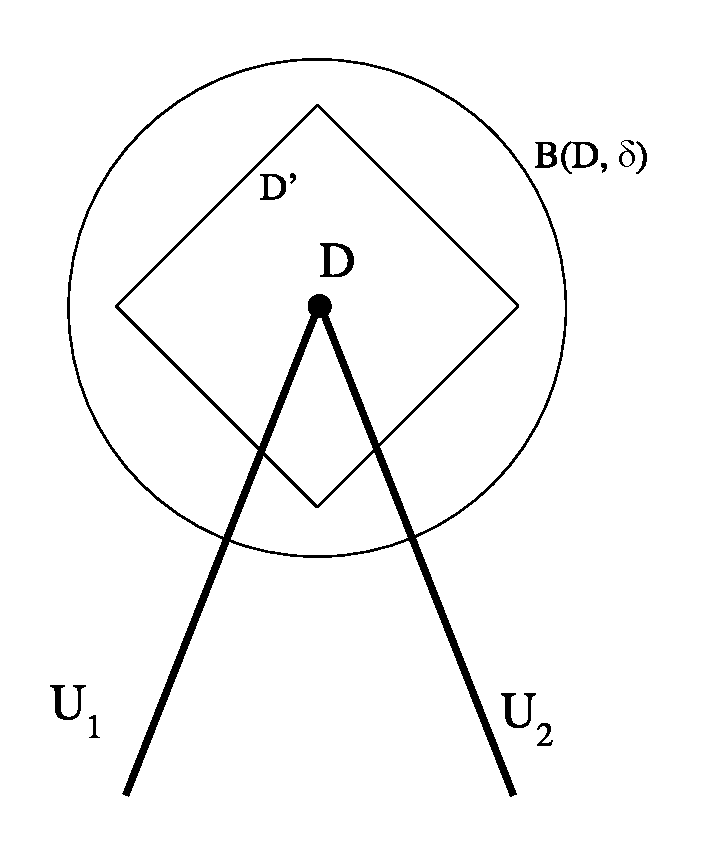
\includegraphics[width=0.24\textwidth]{figs/separated-proof-2} \hfill
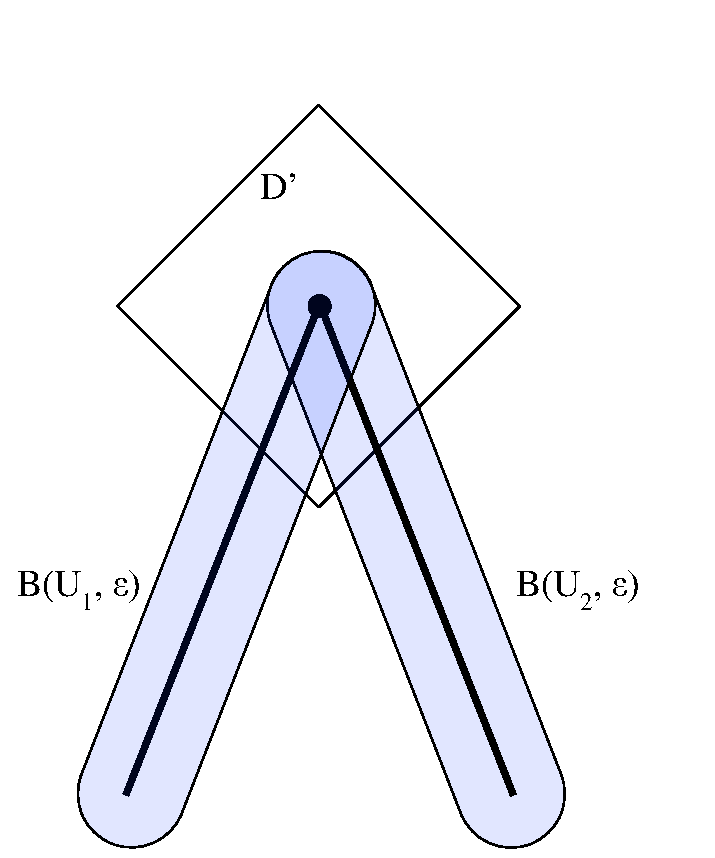
\includegraphics[width=0.24\textwidth]{figs/separated-proof-3} \hfill
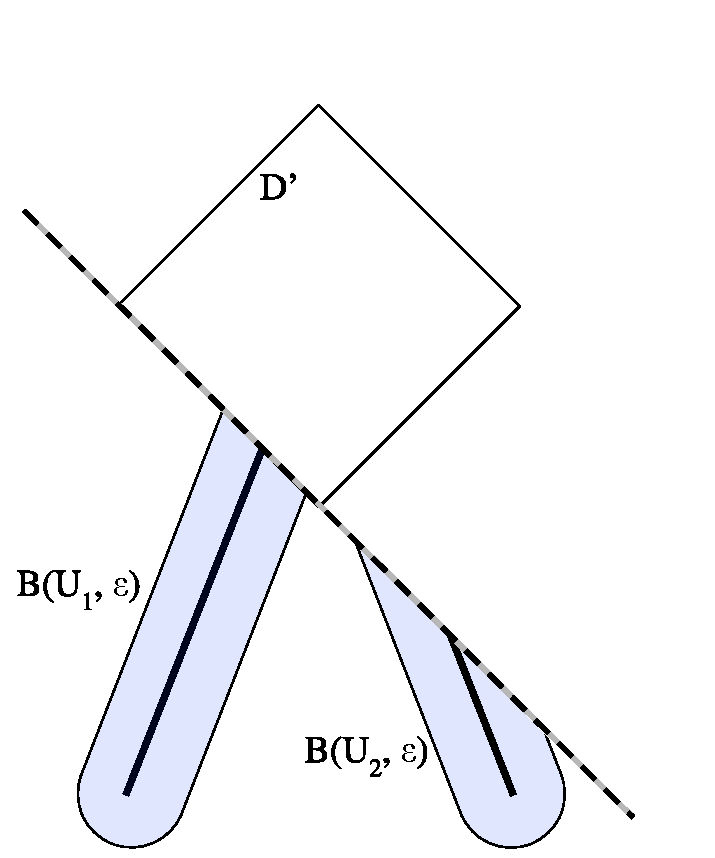
\includegraphics[width=0.24\textwidth]{figs/separated-proof-4} \hfill
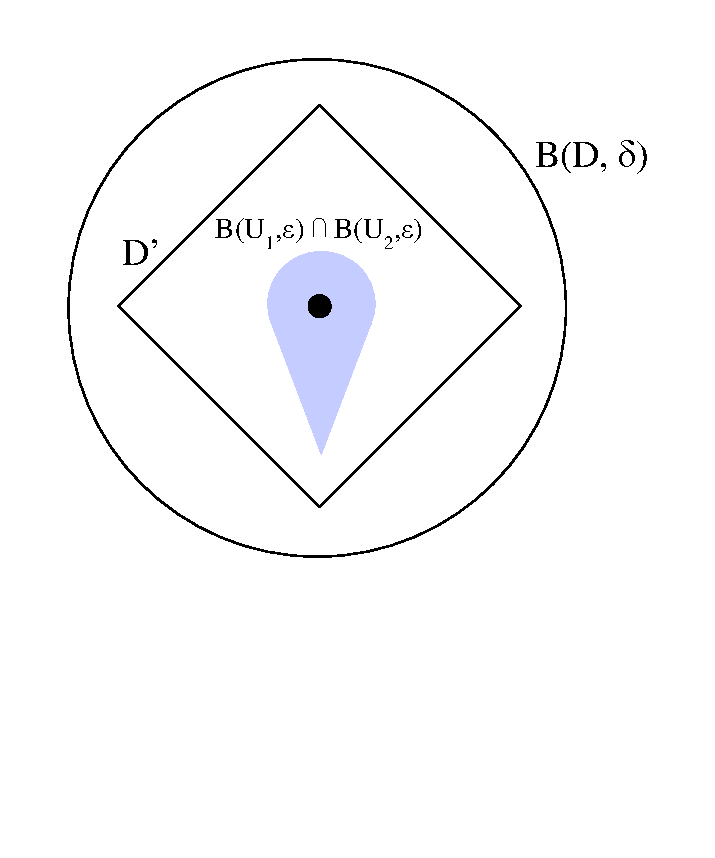
\includegraphics[width=0.24\textwidth]{figs/separated-proof-5}
\end{figure}

\begin{lemma} \label{lemma:thick-empty}
  Let $\{U_j : j \in \mathcal{J}\}$ be a finite collection of nonempty closed, convex sets with $\cap_{j\in\mathcal{J}} U_j = \emptyset$.
  Then for all $\delta > 0$, there exists  $\epsilon > 0$ such that $\cap_{j\in\mathcal{J}} B(U_j,\epsilon) = \emptyset$.
\end{lemma}
\begin{proof}
  By induction on the size of the family.
  Note that the family must have size at least two.
  Let $U_j$ be any set in the family and let $U' = \cap_{j' \neq j} U_{j'}$.
  There are two possibilities.

  The first possibility, which includes the base case where the size of the family is two, is the case $U'$ is nonempty.
  Because $U_j$ and $U'$ are non-intersecting closed convex sets, they are separated by some distance $\epsilon$.
  By Lemma \ref{lemma:thick-nonempty}, for any $\epsilon > 0$, there exists $\delta > 0$ such that $\cap_{j'\neq j} B(U_{j'},\delta) \subseteq B(U', \epsilon/3)$.
  Then we have $B(U_j, \epsilon/3) \cap B(U', \epsilon/3) = \emptyset$.

  The second possibility is that $U'$ is empty.
  This implies we are not in the base case, as the family must have three or more sets.
  By inductive assumption, for small enough $\delta$ we have $\cap_{j' \neq j} B(U_{j'},\delta) = \emptyset$, which proves this case.
\end{proof}
  

\begin{corollary} \label{cor:thick-intersect}
  There exists a small enough $\epsilon > 0$ such that, for any subset $\{U_j : j \in \mathcal{J}\}$ of $\U$, if $\cap_j U_j = \emptyset$, then $\cap_j B(U_j,\epsilon) = \emptyset$.
\end{corollary}
\begin{proof}
  For each subset, Lemma \ref{lemma:thick-empty} gives an $\epsilon$.
  We take the minimum over these finitely many choices.
\end{proof}

\begin{theorem} \label{thm:small-eps-thick}
  For all small enough $\epsilon$, the epsilon-thickened link $\psi$ (Definition \ref{def:eps-thick-link}) is a well-defined link function from $\R'$ to $\R$, i.e. $\psi(u) \neq \bot$ for all $u$.
\end{theorem}
\begin{proof}
  Fix a small enough $\epsilon$ as promised by Corollary \ref{cor:thick-intersect}.
  Consider any $u \in \R'$.
  If $u$ is not in $B(U,\epsilon)$ for any $U \in \U$, then we have $\Psi(u) = \R$, so it is nonempty.
  Otherwise, let $\{U_j : j \in \mathcal{J}\}$ be the family whose thickenings intersect at $u$.
  By Corollary \ref{cor:thick-intersect}, because of our choice of $\epsilon$, the family themselves has nonempty intersection.
  By Lemma \ref{lemma:calibrated-pos}, their corresponding report sets $\{R_j : j \in \mathcal{J}\}$ also intersect at some $r$, so $\Psi(u)$ is nonempty.
\end{proof}  

\begin{lemma} \label{lemma:distance-loss}
  If $L$ is a polyhedral loss, then for each $p$, there exists a constant $c$ such that, for all $u$,
    \[ L(u;p) - \inf_{u^* \in \R'} L(u^*;p) \geq c \cdot d(\Gamma(p),u) . \]
\end{lemma}
\begin{proof}
  Fix $p$ and let $U = \Gamma(p)$.
  If $u \in U$, then both sides are zero.
  So it remains to find a $c$ such that the inequality holds for all $u \not\in U$.

  \bo{Change $\underbar{L}$ to something like $\hat{L}$.}
  
  $L(\cdot;p)$ is a convex polyhedral function, so it is the pointwise maximum over finitely many linear functions.
  Construct the convex polyhedral function $\underbar{L}(\cdot;p)$ by dropping from the max those linear functions that are never equal to $L$ for any $u^* \in U$.
  We have $\underbar{L}(u^*;p) = L(u^*;p)$ for all $u^* \in U$ and $\underbar{L}(u;p) \leq L(u;p)$ for all $u \not\in U$.
  Now $\underbar{L}$ is the max over a finite number of linear functions.
  Each such function $f$ with gradient $\nabla f$ is equal to $\underbar{L}$ above a closed, convex cell in the power diagram formed by projecting $\underbar{L}(\cdot;p)$.
  If $f$ has nonzero gradient, its cell overlaps with $U$ exactly at some face of $U$.
  We will prove that there exists $c_f > 0$ such that, for all $u$ in the corresponding cell of the power diagram,
    \[ \underbar{L}(u;p) \geq L(u^*;p) + c_f \cdot d(U,u) . \]
  We will then repeat this for the finitely many $f$ with nonzero gradient (which covers all points $u \not\in U$) and take the minimum to obtain the desired $c > 0$.

  Consider the set of unit vectors $\{v \in \reals^d : \|v\|=1\}$ and the set of $u^*$ on the boundary of $U$.
  For all pairs $u^*,v$ such that $v$ exposes $u^*$, let
    \[ G_{u^*,v} = \left\{ u^* + \beta v : \beta \geq 0 \right\} . \]
  Note that $\{ u : u \not\in U\} \subseteq \cup_{u^*,v} G_{u^*,v}$.
  We claim each $G_{u^*,v}$ can be associated with some linear $f$ such that $f(u) = \underbar{L}(u;p)$ for all $u \in G_{u^*,v}$.
  \bo{Need to prove this; I think it follows because $G_{u^*,v}$ lies completely within some cell of the power diagram formed by projecting $\underbar{L}$.}
  Hence for all $u$ in $G_{u^*,v}$, we have
  \begin{align*}
    \underbar{L}(u;p) &= \underbar{L}(u^*;p) + (\nabla f) \cdot (d(u^*,u) v)  \\
                      &= L(u^*;p) + c_{u^*,v} \cdot d(U,u)
  \end{align*}
  where $c_{u^*,v} := (\nabla f) \cdot v$, and we note $u^* = \min_{u' \in U} d(u',u)$. \bo{Should prove this; ought to follow because $v$ exposes $u^*$.}
  We must have $c_{u^*,v} > 0$, otherwise $G_{u^*,v} \subseteq U$ which is a contradiction.
  
  Now for each $f$, we claim the set $\{u^*, v : \text{$G_{u^*,v}$ is associated with $f$}\}$ is closed.
  This follows because the set of $u^*$ such that $f(u^*) = \underbar{L}(u^*;p)$ is closed, and for fixed $u^*$, the set of $v$ such that $G_{u^*,v}$ is in the cell of the power diagram is also closed.\bo{Should prove this.}
  So for this $f$, the infimum over all positive $c_{u^*,v}$ is achieved by some positive member $c_f > 0$.
\end{proof}

\begin{theorem} \label{thm:app-eps-thick-sep}
  For small enough $\epsilon$, the $\epsilon$-thickened link $\psi$ (Definition \ref{def:eps-thick-link}) satisfies that, for all $p$, there exists $\delta > 0$ such that, for all $u \in \R'$,
    \[ L(u;p) - \inf_{u^* \in \R'} L(u^*;p) \geq \delta \left[ \ell(\psi(u);p) - \min_{r^* \in \R} \ell(r^*;p) \right] . \]
\end{theorem}
\begin{proof}
  We take the $\epsilon$ thickened link, which is well-defined by Theorem \ref{thm:small-eps-thick}.
  Fix $p$ and let $U = \Gamma(p)$.
  The left-hand side is nonnegative, so it suffices to prove the result for all $u$ such that the right side is strictly positive, i.e. for all $u$ such that $\psi(u) \not\in \gamma(p)$.
  By definition of the $\epsilon$-thickened link, we must have $d(U,u) \geq \epsilon$.
  By Lemma \ref{lemma:distance-loss}, we have $L(u;p) - \inf_{u^*} L(u^*;p) \geq C$ where $C = c\epsilon$ for some $c > 0$.
  This holds for all $u$.
  Meanwhile,
    \[ \ell(\psi(u);p) - \min_{r^*} \ell(r^*;p) \leq \max_{r \in \R} \ell(r;p) - \min_{r^* \in \R} \ell(r^*;p) =: D, \]
  for some constant $D$.
  This also holds for all $u$.
  Set $\delta = \frac{C}{D}$ to complete the proof.
\end{proof}

\begin{proof}[Proof of Theorem \ref{thm:eps-thick-calibrated}]
  The two claims are Theorems \ref{thm:small-eps-thick} and \ref{thm:app-eps-thick-sep}.
\end{proof}


\section{Top-$k$ surrogate}
Throughout this section, consider the surrogate and discrete loss $L_2(u,y)~:=~\left(\frac{1}{k} \sum_{i=1}^k (u + \ones - e_y)_{[i]} - u_y \right)_+$ and $\ell_2(r,y) = \Ind{y \not\in r} + \frac{|r \setminus \{y\}|}{k}$ given in Equations~\ref{eq:L-2-surrogate} and~\ref{eq:ell-2}, respectively.


Observe that $L_2$ is a polyhedral loss, since it can be written as the pointwise max of $\binom{n}{k} +1$ terms, where the $\binom{n}{k}$ terms are selecting the $k$ elements of $u + \ones - e_y$ with highest weight.
By Lemma~\ref{lem:poly-loss-poly-risk}, we then know that $\risk{L_2}$ is also polyhedral.

\begin{lemma}\label{lem:top-k-optimal-corners}
	For all $p \in \simplex$, there is a $u \in \{ u \in \{0,1\}^n : \|u\|_1 \leq k\}$ such that $u \in \argmin_{u' \in \reals^d} \inprod{p}{L_2(u)}$.
\end{lemma}
\begin{proof}[Sketch]
  First, observe that $L_2$ is invariant in the $\ones$ direction, so without loss of generality, we can restrict our consideration to reports so that $u_{[n]} = 0$.
  
  We first claim that for all $y \in \Y$, the minimum of $L(u)_y$ is achieved by some $u \in [0,1]^n$.
  Observe that if $u_{[1]} \geq u_{[n]} + 1$, the value of the loss gets ``cropped'' and will be the same by reporting $u_{[1]} = u_{[n]} + 1 = 1$. \jessiet{Flesh this out later.}
  Since $u_{[n]} = 0 \implies u_{[1]} \in [0,1]$, we can then observe there is some $u \in \prop{L_2}$ so that $u \in [0,1]^n$.
    
  Now, since we can restrict to the closed hypercube, we claim that we can rewrite the surrogate $L_2$ as 
  \begin{align*}
  	\inprod{p}{L_2(u)} &:= \frac{1}{k} \left( \sum_{i=1}^k (1 - p_{[i]}) u_{[i]} + u_{[k+1]} \sum_{i=1}^k p_{[i]} \right) + 1 - \inprod{p}{u}
  \end{align*}
  
  To verify this, observe the first term of the summation comes from the probability that you incorrectly did not have $u_y$ in the top-$k$, and the second term comes from the $(k+1)^{th}$ term being added when $u_y$ is correctly in the top $k$ (and therefore not an averaged term, since $u_y \in [0,1]$.) 
  The $1$ is pulled out from the average, and $\inprod{p}{u}$ comes from the $-u_y$ term form each $y$ by linearity of expectation.
  We don't need to concern ourselves with the max operator since $\frac{1}{k} \sum_{i=1}^k (u + \ones - e_y)_{[i]} - u_y \geq 0$ for all $y \in \Y$ on $[0,1]^n$.
  
  Since, for $u_{[j]}$ and $j \geq k+2$, the expected loss only decreases by increasing $u_{[j]}$ as much as possible, we increase them to $u_{[k+1]}$.
  By our invariance in the $\ones$ direction, we can re-shift our values if necessary, setting $u_{[k+1]} = u_{[k+2]} = \ldots = u_{[n]} = 0$.
  
  Substituting these values into the expected loss, we now observe a linear objective over the hypercube, which is known to be optimal on some corner of the hypercube, so the rest of $u_{[1]}, u_{[2]}, \ldots, u_{[k]} \in \{0,1\}$.
  Therefore, for all $p \in \simplex$, there is a report $u \in \{0,1\}^n$ optimizing $L_2$.
  Moreover, for this optimal $u$, observe $\|u\|_{1} \leq k$ since we have $u_{[k+1]} = u_{[k+2]} = \ldots = u_{[n]} = 0$.
\end{proof}

\begin{lemma}\label{lem:top-k-surrogate-embeds}
$L_2:\reals^n \to \reals^\Y_+$ embeds $\ell_2:\R \to \reals^\Y_+$.
\end{lemma}
\begin{proof}
  We can verify $\ell_2(r) = L_2(\varphi(r))$ for all $r \subseteq [n]$ and $\varphi(r)$ being its conversion from a set to binary vector, so $\varphi(\R) = \{ u \in \{0,1\}^n : \|u\|_1 \leq k \}$.
  Moreover, by Lemma~\ref{lem:top-k-optimal-corners} and the above equality, respectively, we know that $\inf_{u \in \reals^n} \inprod{p}{L_2(u)} = \min_{u \in \varphi(\R)} \inprod{p}{L_2(u)} = \min_{r \in \R}\inprod{p}{\ell_2(r)}$ for all $p \in \simplex$, and so we conclude that $L_2$ embeds $\ell_2$.
\end{proof}


\end{document}
%%% Local Variables:
%%% mode: latex
%%% TeX-master: t
%%% End:
